\documentclass[]{book}
\usepackage{lmodern}
\usepackage{amssymb,amsmath}
\usepackage{ifxetex,ifluatex}
\usepackage{fixltx2e} % provides \textsubscript
\ifnum 0\ifxetex 1\fi\ifluatex 1\fi=0 % if pdftex
  \usepackage[T1]{fontenc}
  \usepackage[utf8]{inputenc}
\else % if luatex or xelatex
  \ifxetex
    \usepackage{mathspec}
  \else
    \usepackage{fontspec}
  \fi
  \defaultfontfeatures{Ligatures=TeX,Scale=MatchLowercase}
\fi
% use upquote if available, for straight quotes in verbatim environments
\IfFileExists{upquote.sty}{\usepackage{upquote}}{}
% use microtype if available
\IfFileExists{microtype.sty}{%
\usepackage[]{microtype}
\UseMicrotypeSet[protrusion]{basicmath} % disable protrusion for tt fonts
}{}
\PassOptionsToPackage{hyphens}{url} % url is loaded by hyperref
\usepackage[unicode=true]{hyperref}
\hypersetup{
            pdftitle={卒業論文のためのR入門},
            pdfauthor={森 知晴(立命館大学総合心理学部)},
            pdfborder={0 0 0},
            breaklinks=true}
\urlstyle{same}  % don't use monospace font for urls
\usepackage{natbib}
\bibliographystyle{apalike}
\usepackage{color}
\usepackage{fancyvrb}
\newcommand{\VerbBar}{|}
\newcommand{\VERB}{\Verb[commandchars=\\\{\}]}
\DefineVerbatimEnvironment{Highlighting}{Verbatim}{commandchars=\\\{\}}
% Add ',fontsize=\small' for more characters per line
\usepackage{framed}
\definecolor{shadecolor}{RGB}{248,248,248}
\newenvironment{Shaded}{\begin{snugshade}}{\end{snugshade}}
\newcommand{\KeywordTok}[1]{\textcolor[rgb]{0.13,0.29,0.53}{\textbf{#1}}}
\newcommand{\DataTypeTok}[1]{\textcolor[rgb]{0.13,0.29,0.53}{#1}}
\newcommand{\DecValTok}[1]{\textcolor[rgb]{0.00,0.00,0.81}{#1}}
\newcommand{\BaseNTok}[1]{\textcolor[rgb]{0.00,0.00,0.81}{#1}}
\newcommand{\FloatTok}[1]{\textcolor[rgb]{0.00,0.00,0.81}{#1}}
\newcommand{\ConstantTok}[1]{\textcolor[rgb]{0.00,0.00,0.00}{#1}}
\newcommand{\CharTok}[1]{\textcolor[rgb]{0.31,0.60,0.02}{#1}}
\newcommand{\SpecialCharTok}[1]{\textcolor[rgb]{0.00,0.00,0.00}{#1}}
\newcommand{\StringTok}[1]{\textcolor[rgb]{0.31,0.60,0.02}{#1}}
\newcommand{\VerbatimStringTok}[1]{\textcolor[rgb]{0.31,0.60,0.02}{#1}}
\newcommand{\SpecialStringTok}[1]{\textcolor[rgb]{0.31,0.60,0.02}{#1}}
\newcommand{\ImportTok}[1]{#1}
\newcommand{\CommentTok}[1]{\textcolor[rgb]{0.56,0.35,0.01}{\textit{#1}}}
\newcommand{\DocumentationTok}[1]{\textcolor[rgb]{0.56,0.35,0.01}{\textbf{\textit{#1}}}}
\newcommand{\AnnotationTok}[1]{\textcolor[rgb]{0.56,0.35,0.01}{\textbf{\textit{#1}}}}
\newcommand{\CommentVarTok}[1]{\textcolor[rgb]{0.56,0.35,0.01}{\textbf{\textit{#1}}}}
\newcommand{\OtherTok}[1]{\textcolor[rgb]{0.56,0.35,0.01}{#1}}
\newcommand{\FunctionTok}[1]{\textcolor[rgb]{0.00,0.00,0.00}{#1}}
\newcommand{\VariableTok}[1]{\textcolor[rgb]{0.00,0.00,0.00}{#1}}
\newcommand{\ControlFlowTok}[1]{\textcolor[rgb]{0.13,0.29,0.53}{\textbf{#1}}}
\newcommand{\OperatorTok}[1]{\textcolor[rgb]{0.81,0.36,0.00}{\textbf{#1}}}
\newcommand{\BuiltInTok}[1]{#1}
\newcommand{\ExtensionTok}[1]{#1}
\newcommand{\PreprocessorTok}[1]{\textcolor[rgb]{0.56,0.35,0.01}{\textit{#1}}}
\newcommand{\AttributeTok}[1]{\textcolor[rgb]{0.77,0.63,0.00}{#1}}
\newcommand{\RegionMarkerTok}[1]{#1}
\newcommand{\InformationTok}[1]{\textcolor[rgb]{0.56,0.35,0.01}{\textbf{\textit{#1}}}}
\newcommand{\WarningTok}[1]{\textcolor[rgb]{0.56,0.35,0.01}{\textbf{\textit{#1}}}}
\newcommand{\AlertTok}[1]{\textcolor[rgb]{0.94,0.16,0.16}{#1}}
\newcommand{\ErrorTok}[1]{\textcolor[rgb]{0.64,0.00,0.00}{\textbf{#1}}}
\newcommand{\NormalTok}[1]{#1}
\usepackage{longtable,booktabs}
% Fix footnotes in tables (requires footnote package)
\IfFileExists{footnote.sty}{\usepackage{footnote}\makesavenoteenv{long table}}{}
\usepackage{graphicx,grffile}
\makeatletter
\def\maxwidth{\ifdim\Gin@nat@width>\linewidth\linewidth\else\Gin@nat@width\fi}
\def\maxheight{\ifdim\Gin@nat@height>\textheight\textheight\else\Gin@nat@height\fi}
\makeatother
% Scale images if necessary, so that they will not overflow the page
% margins by default, and it is still possible to overwrite the defaults
% using explicit options in \includegraphics[width, height, ...]{}
\setkeys{Gin}{width=\maxwidth,height=\maxheight,keepaspectratio}
\IfFileExists{parskip.sty}{%
\usepackage{parskip}
}{% else
\setlength{\parindent}{0pt}
\setlength{\parskip}{6pt plus 2pt minus 1pt}
}
\setlength{\emergencystretch}{3em}  % prevent overfull lines
\providecommand{\tightlist}{%
  \setlength{\itemsep}{0pt}\setlength{\parskip}{0pt}}
\setcounter{secnumdepth}{5}
% Redefines (sub)paragraphs to behave more like sections
\ifx\paragraph\undefined\else
\let\oldparagraph\paragraph
\renewcommand{\paragraph}[1]{\oldparagraph{#1}\mbox{}}
\fi
\ifx\subparagraph\undefined\else
\let\oldsubparagraph\subparagraph
\renewcommand{\subparagraph}[1]{\oldsubparagraph{#1}\mbox{}}
\fi

% set default figure placement to htbp
\makeatletter
\def\fps@figure{htbp}
\makeatother

\usepackage{booktabs}

\title{卒業論文のためのR入門}
\author{森 知晴(立命館大学総合心理学部)}
\date{Last Update: 2020-09-03}

\begin{document}
\maketitle

{
\setcounter{tocdepth}{1}
\tableofcontents
}
\chapter{はじめに}\label{Introduction}

この文書は、卒業論文を書くためのRの使い方を\textbf{できるだけコンパクトに}まとめたものです。
読者は立命館大学総合心理学部森ゼミの学生をピンポイントに想定しています。

\begin{itemize}
\tightlist
\item
  Rを用いた演習として「心理学データ解析法」の履修を推奨していますが、履修していなくてもわかるように構成しています。
\item
  卒業論文自体はWordで作成する想定で、Rで得られた結果をWordに貼り付ける(簡便な)方法を説明します。
\end{itemize}

一般的なRの入門文書としても参照できます。
説明の都合上、厳密さよりわかりやすさを重視した記述が多々あります。ご了承ください。

具体的には、以下の項目を学習します。

\begin{itemize}
\tightlist
\item
  R, RStudioをインストールし、基本的な操作ができるようになる
\item
  データをRStudioにインポートする
\item
  インポートしたデータを分析可能な形に前処理する
\item
  記述統計を整理する
\item
  データを可視化する
\item
  t検定を行う
\item
  重回帰分析を行い、論文に貼り付けられる形に整える
\end{itemize}

文書は前から順番に読み、自分でコードを打って確かめてください。 Chapter
\ref{InstallR}を読んでRとRStudioを準備し、登場するコードを自分で入力して練習してみてください。

この文書で紹介している方法はあくまで一例です。
Rには様々な機能やパッケージがあり、日々進化しています。
この文書の内容を理解したら、ぜひ自分で様々な機能を調べて使ってみてください!

★参考文献

\begin{itemize}
\tightlist
\item
  浅野正彦・中村公亮(2018)はじめてのRStudio
  エラーメッセージなんてこわくない、オーム社
\item
  松村優哉・湯谷啓明・紀ノ定保礼・前田和寛(2018)RユーザのためのRStudio{[}実践{]}入門
  −tidyverseによるモダンな分析フローの世界−
\end{itemize}

\chapter{R(Studio)のインストール}\label{InstallR}

R(Studio)のインストールは最大の難関となる可能性があります(特にWindowsの場合)。
紹介するマニュアルを丁寧に読んでインストールしてください。

インストール方法は高知工科大学の矢内勇生先生のサイトで紹介されているので、そちらをご覧ください。

\url{http://yukiyanai.github.io/jp/resources/}

インストールのポイント(Windows)

\begin{itemize}
\tightlist
\item
  矢内先生のスライドを丁寧に読み一つ一つ手順を追って進める

  \begin{itemize}
  \tightlist
  \item
    インストール1(プログラミング用フォント)はわからなければスキップしても良い
  \item
    インストール4(Rtools)はスキップする
  \item
    RStudioのカスタマイズはスキップする
  \end{itemize}
\item
  ディレクトリ(フォルダ)の名前に日本語(中国語・韓国語)が含まれている場合、大きな問題となり得る
  → 対処法をよく読む
\item
  OneDriveでのバックアップ機能が使われている場合、大きな問題となり得る →
  対処法をよく読む
\end{itemize}

インストールのポイント(macOS)

\begin{itemize}
\tightlist
\item
  矢内先生のスライドを丁寧に読み一つ一つ手順を追って進める

  \begin{itemize}
  \tightlist
  \item
    RStudioのカスタマイズはスキップする
  \end{itemize}
\end{itemize}

資料を読んで操作してもよくわからなかった場合、森の授業・ゼミの受講生は連絡してください。

\chapter{RStudioの使い方}\label{RStudio}

\section{RStudioの起動}\label{rstudioux306eux8d77ux52d5}

それでは、RStudioを起動してみましょう。
正しくインストールされていれば、Windowsはスタートメニュー、Macの場合はアプリケーションのアイコンをクリックして起動できるはずです。
R本体はインストールされていればOKです。自分で起動する必要はありません。

RStudioは今後何度も起動するので、ショートカットを作ってデスクトップから起動できるようにしておくと便利です。

\section{RStudioの画面}\label{rstudioux306eux753bux9762}

人によって多少異なりますが、RStudioを起動した画面は以下のようになっています。

\begin{center}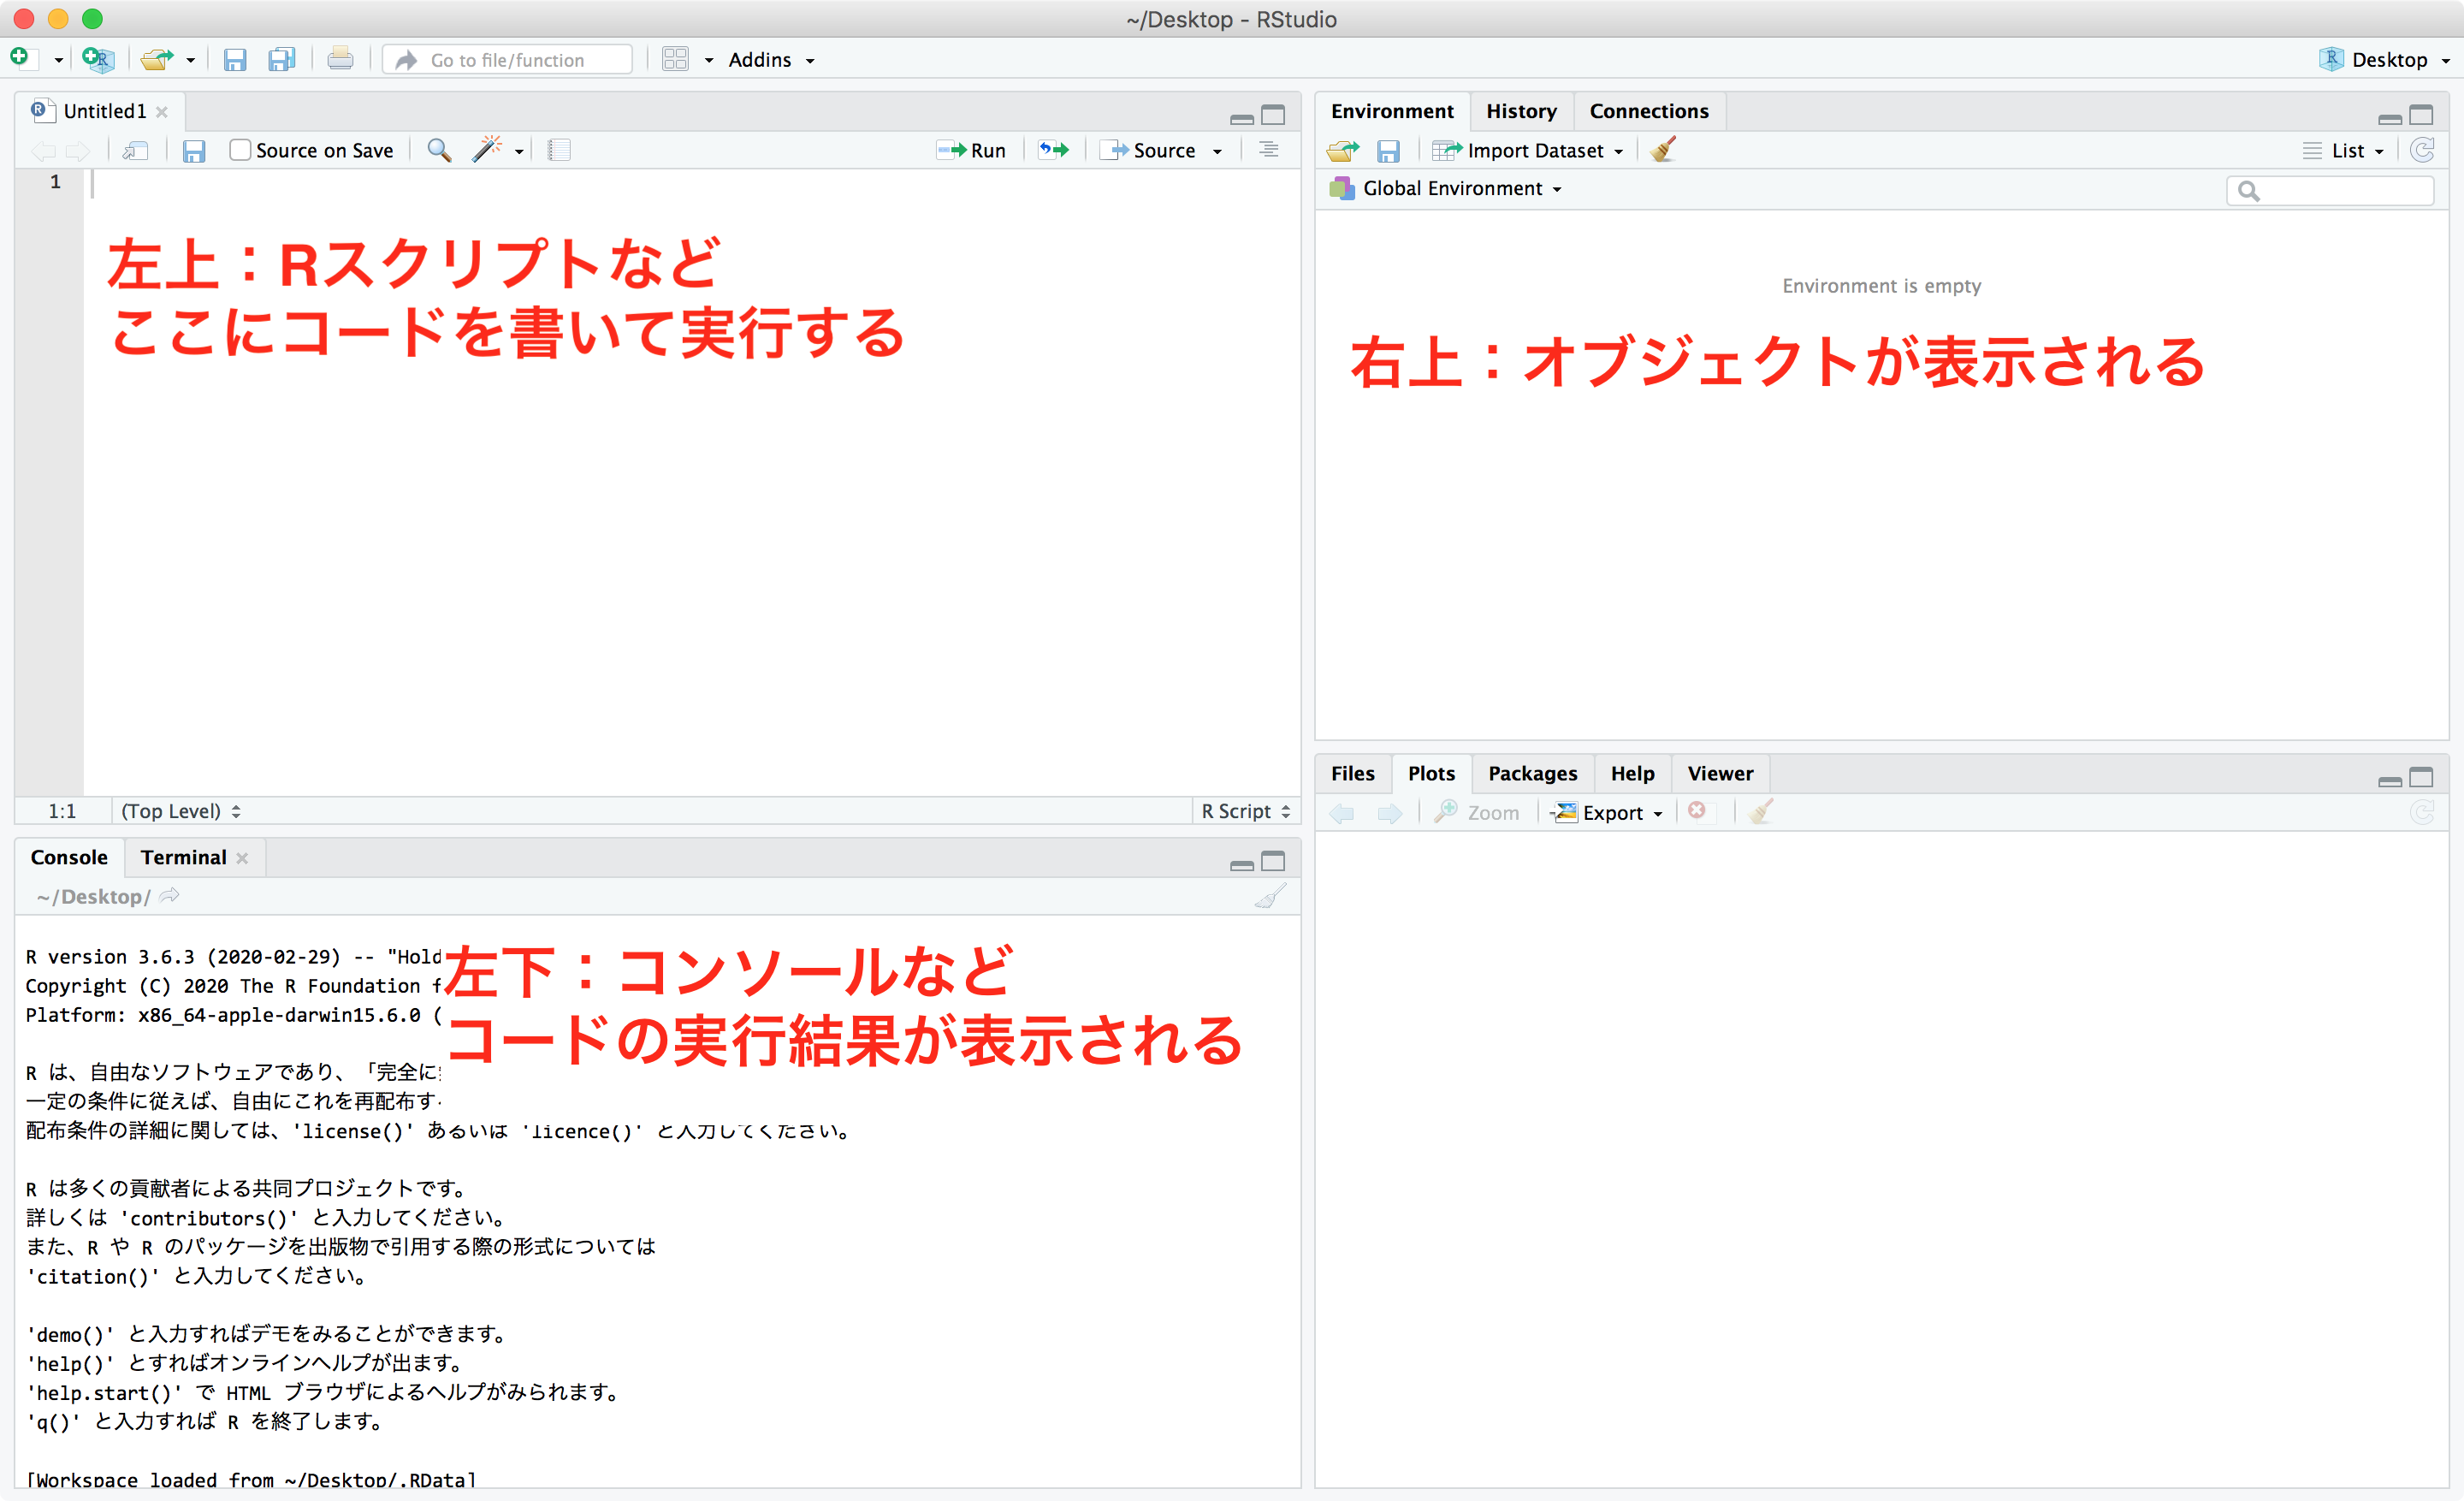
\includegraphics[width=0.7\linewidth]{image/RStudio_screen} \end{center}

RStudioは通常4つのウィンドウ(ペーンと呼びます)に分割されます。
ここでは各ペーンの概要を説明します。

\begin{itemize}
\tightlist
\item
  左上のペーンはRStudioを動かすためのコードを書く場所です。表示されていなければ、左上の緑の+をクリックし、「R
  Script」を選択してください。
\item
  左下のペーンはコンソールと呼ばれる、コードの実行結果を表示する場所です。ここに直接コードを書くこともできますが、コードは保存されません。
\item
  右上のペーンは後述する「オブジェクト」が表示される場所です。
\item
  右下のペーンはファイルやパッケージなどが表示される場所です。
\end{itemize}

\section{RStudioの操作}\label{rstudioux306eux64cdux4f5c}

それでは、実際に操作してみましょう。Rスクリプトに\texttt{1\ +\ 1}と打ってみてください。

\begin{center}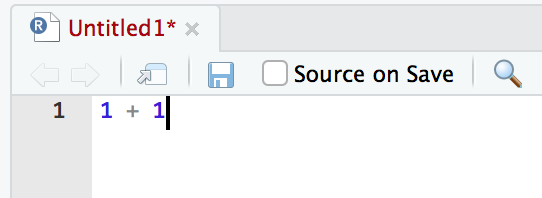
\includegraphics[width=0.4\linewidth]{image/basic1} \end{center}

これが1行のコードになります。この行にカーソルを合わせた状態で、WindowsではCtrl
+ Enter、MacではCommand + Enterを押してください。
(スクリプト右上のRunを押しても良いです)

\begin{center}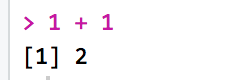
\includegraphics[width=0.2\linewidth]{image/basic2} \end{center}

すると、コンソールに結果が表示されました。\textgreater{} 1 +
1は実行したコードを表しています。
{[}1{]}は行番号を表します。その右側が結果です。

もう少しコードを書いてみましょう。\texttt{3\ -\ 1} \texttt{2\ *\ 3}
\texttt{6\ /\ 2}と3行のコードを書いてください。

\begin{center}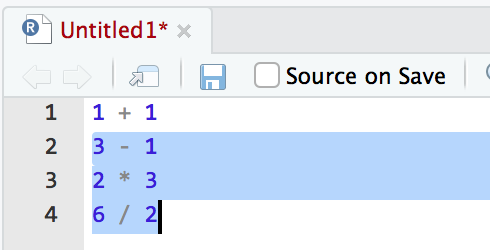
\includegraphics[width=0.4\linewidth]{image/basic3} \end{center}

これをまとめて選択してCtrl + Enter (Command + Enter)を押してください。

\begin{center}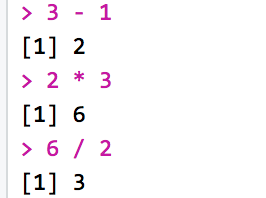
\includegraphics[width=0.2\linewidth]{image/basic4} \end{center}

すると、それぞれの計算結果が表示されました。

スクリプトにコードを書く→実行してコンソールで結果を確認、という一連の作業を繰り返して慣れていきましょう。

\section{スクリプトの保存}\label{ux30b9ux30afux30eaux30d7ux30c8ux306eux4fddux5b58}

スクリプトはWindowsはCtrl + S、MacはCommand +
Sで保存することができます。
スクリプトを保存しておけば、次回に書き直す必要はありません。
卒業論文では、何度もスクリプトを書き直すので、きちんと保存しておきましょう。

\section{プロジェクトの作成}\label{ux30d7ux30edux30b8ux30a7ux30afux30c8ux306eux4f5cux6210}

RStudioには「プロジェクト」という機能があり、これを使うとファイル管理がしやすくなります。
プロジェクトはコンピュータ内にフォルダを作成し(または既存のフォルダを指定し)、そのフォルダの中で作業を行います。

プロジェクトを作成してみましょう。
左上の左から2つ目の緑の+を押してください。

\begin{center}
\includegraphics[width=0.05\linewidth]{image/project1} \end{center}

表示されるウィンドウで、``New Directory''を選んでください。

\begin{center}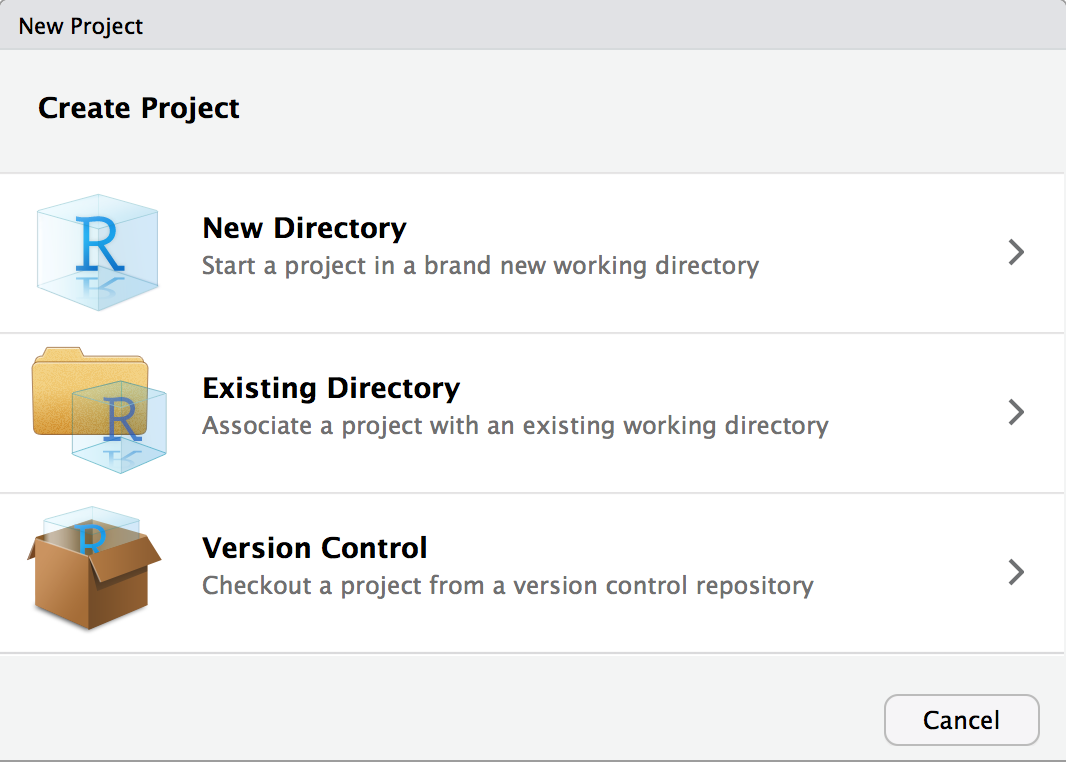
\includegraphics[width=0.5\linewidth]{image/project2} \end{center}

次のウィンドウでは、``New Project''を選んでください。

\begin{center}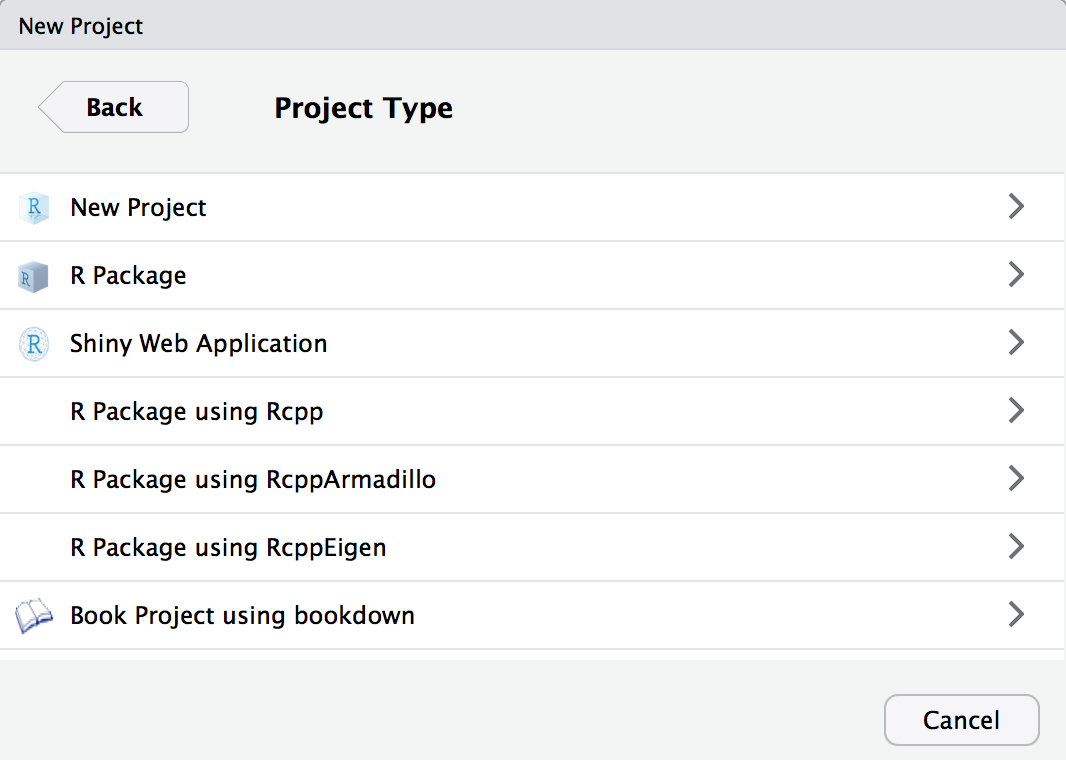
\includegraphics[width=0.5\linewidth]{image/project3} \end{center}

次の画面で作成するフォルダ名(プロジェクト名になります)とフォルダの作成場所を指定します。
\textbf{フォルダ名は英数字のみとしてください。フォルダを作成する場所も英数字となるような場所にしてください。}

指定したら、Create Projectを押してプロジェクトを作成してください。

\begin{center}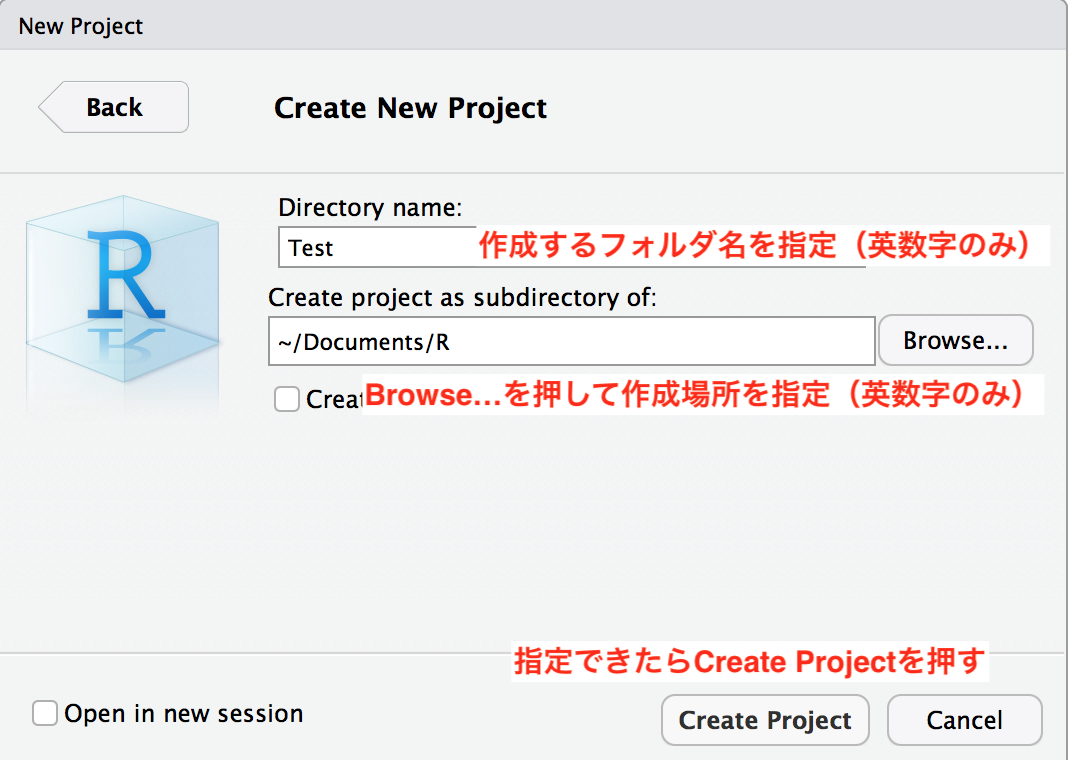
\includegraphics[width=0.5\linewidth]{image/project4} \end{center}

コンピュータで指定したフォルダに行き、フォルダが新たに作成されていること、{[}プロジェクト名.Rproj{]}というファイルが中に作成されていることを確認してください。

\begin{center}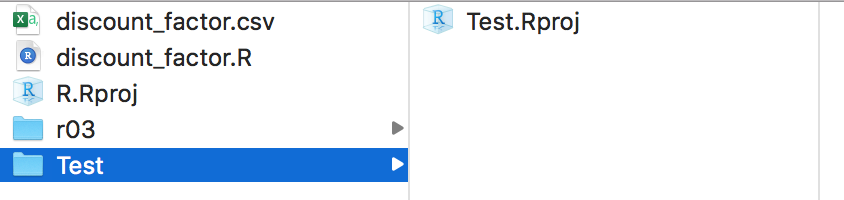
\includegraphics[width=0.5\linewidth]{image/project5} \end{center}

Testというフォルダが新たに作られ、中にTest.Rprojというファイルが入っています。

RStudioを使う際は、プロジェクトをベースに作業するようにしましょう。

\begin{itemize}
\tightlist
\item
  起動の際は、プロジェクト名.Rprojをクリックして起動する。
\item
  使用するファイルは、プロジェクトのフォルダに移動・保存するようにする。
\item
  RStudioでファイルを作成した場合、このフォルダに保存されます。
\end{itemize}

試しに、新しいRスクリプトを作成(左上の緑の+を押す)し、保存して見てください。
フォルダ内にRスクリプト(.Rで終わるファイル)ができていれば成功です。

\chapter{パッケージのインストール}\label{Packages}

Rの機能を拡張するため、必要なパッケージをインストールします。
まずは、重要なパッケージがまとめられている\texttt{tidyverse}(読み:タイディバース)をインストールしましょう。
その他のパッケージは必要になる度に紹介します。

\begin{Shaded}
\begin{Highlighting}[]
\KeywordTok{install.packages}\NormalTok{(}\StringTok{"tidyverse"}\NormalTok{)}
\KeywordTok{library}\NormalTok{(tidyverse)}
\end{Highlighting}
\end{Shaded}

\texttt{install.packages()}は各パソコンで一度実行すればOKです。
\texttt{library()}はRStudioを起動するたびに実行する必要があります。
Rスクリプトの冒頭に使用する\texttt{library()}を並べておき、起動するたびに実行するようにしましょう。

確認のため、以下のコードを打って、動作するかどうか確認してみてください。
(データセット\texttt{mtcars}の変数\texttt{mpg}の平均を計算するコードです)

\begin{Shaded}
\begin{Highlighting}[]
\NormalTok{mtcars }\OperatorTok\StringTok{ }\KeywordTok{summarize}\NormalTok{(}\DataTypeTok{mean_mpg =} \KeywordTok{mean}\NormalTok{(mpg))}
\end{Highlighting}
\end{Shaded}

\begin{verbatim}
##   mean_mpg
## 1 20.09062
\end{verbatim}

ここでエラーが起きた場合、R(Studio)のインストールがうまくいっていない可能性があります。
Chapter \ref{InstallR}に戻って確認しましょう。

\begin{Shaded}
\begin{Highlighting}[]
\KeywordTok{library}\NormalTok{(tidyverse)}
\end{Highlighting}
\end{Shaded}

\chapter{Rの基本操作}\label{Rbasics}

\section{オブジェクト}\label{ux30aaux30d6ux30b8ux30a7ux30afux30c8}

Rで使用するあらゆる「モノ」はオブジェクト(object)と呼ばれ管理されます。
オブジェクトの準備からRの分析はスタートします。まずは、オブジェクトを準備してみましょう。

\begin{Shaded}
\begin{Highlighting}[]
\NormalTok{first_object <-}\StringTok{ }\DecValTok{1} 
\end{Highlighting}
\end{Shaded}

オブジェクトは「名前」と「中身」で構成されます。
このコマンドでは、\texttt{first\_object}という名前のオブジェクトに「1」という数値を入れています。
\texttt{\textless{}-}(不等号・ハイフン)は矢印を表していて、左側の名前のオブジェクトに右側の「モノ」を代入する命令です。
このコマンドを実行しても何も表示されませんが、それでOKです。

オブジェクトの名前を指定すると、オブジェクトの中身を表示させることができます。

\begin{Shaded}
\begin{Highlighting}[]
\NormalTok{first_object}
\end{Highlighting}
\end{Shaded}

\begin{verbatim}
## [1] 1
\end{verbatim}

{[}1{]}は「1行目」を意味しています。そのあとの「1」が中身です。

また、代入する命令を\texttt{()}でくくることで、代入させつつ表示させることができます。
\texttt{second\_object}に2を入れて表示させてみましょう。

\begin{Shaded}
\begin{Highlighting}[]
\NormalTok{(second_object <-}\StringTok{ }\DecValTok{2}\NormalTok{)}
\end{Highlighting}
\end{Shaded}

\begin{verbatim}
## [1] 2
\end{verbatim}

文字列をオブジェクトに入れることもできます。
この場合、文字列を``''(引用符)でくくります。

\begin{Shaded}
\begin{Highlighting}[]
\NormalTok{first_string_object <-}\StringTok{ "Ritsumeikan University"}
\NormalTok{first_string_object}
\end{Highlighting}
\end{Shaded}

\begin{verbatim}
## [1] "Ritsumeikan University"
\end{verbatim}

ここでは、\texttt{first\_string\_object}という名前のオブジェクトに、文字列\texttt{"Ritsumeikan\ University"}を入れています。

オブジェクトに入れるものは1つの値ではなく、複数の値にすることもできます。
複数の値を並べたものは「ベクトル」と呼ばれます。
ベクトルは\texttt{c()}でまとめます。

\begin{Shaded}
\begin{Highlighting}[]
\NormalTok{first_vector_object <-}\StringTok{ }\KeywordTok{c}\NormalTok{(}\DecValTok{1}\NormalTok{, }\DecValTok{2}\NormalTok{, }\DecValTok{3}\NormalTok{, }\DecValTok{4}\NormalTok{, }\DecValTok{5}\NormalTok{)}
\NormalTok{first_vector_object}
\end{Highlighting}
\end{Shaded}

\begin{verbatim}
## [1] 1 2 3 4 5
\end{verbatim}

ここでは、\texttt{first\_vector\_object}というオブジェクトに、1から5までの数値を代入しています。
文字列のベクトルも作ることができるので、試してみてください。

★練習問題

\begin{itemize}
\tightlist
\item
  \texttt{third\_object}という名前のオブジェクトに\texttt{10000}を代入し、確認してください。
\item
  \texttt{my\_name}という名前のオブジェクトにあなたの名前(文字列)を代入し、確認してください。
\item
  \texttt{second\_vector\_object}という名前のオブジェクトに数値のベクトル\texttt{1,\ 1,\ 2,\ 3,\ 5,\ 8}を代入し、確認してください。
\end{itemize}

\section{簡単な計算}\label{ux7c21ux5358ux306aux8a08ux7b97}

Rでの簡単な計算をしてみましょう。足し算・引き算は日常用語と同じく\texttt{+},
\texttt{-}を用います。

\begin{Shaded}
\begin{Highlighting}[]
\DecValTok{1} \OperatorTok{+}\StringTok{ }\DecValTok{1}
\end{Highlighting}
\end{Shaded}

\begin{verbatim}
## [1] 2
\end{verbatim}

\begin{Shaded}
\begin{Highlighting}[]
\DecValTok{5} \OperatorTok{-}\StringTok{ }\DecValTok{2}
\end{Highlighting}
\end{Shaded}

\begin{verbatim}
## [1] 3
\end{verbatim}

掛け算は\texttt{*}、割り算は\texttt{/}を使います。また、累乗は\texttt{\^{}}です。日常用語とは異なりますが、Excelと同じです。

\begin{Shaded}
\begin{Highlighting}[]
\DecValTok{2} \OperatorTok{*}\StringTok{ }\DecValTok{3}
\end{Highlighting}
\end{Shaded}

\begin{verbatim}
## [1] 6
\end{verbatim}

\begin{Shaded}
\begin{Highlighting}[]
\DecValTok{10} \OperatorTok{/}\StringTok{ }\DecValTok{2}
\end{Highlighting}
\end{Shaded}

\begin{verbatim}
## [1] 5
\end{verbatim}

\begin{Shaded}
\begin{Highlighting}[]
\DecValTok{4} \OperatorTok{^}\StringTok{ }\DecValTok{2}
\end{Highlighting}
\end{Shaded}

\begin{verbatim}
## [1] 16
\end{verbatim}

ここまでは数値同士で計算させていましたが、数値を代入したオブジェクトも使うことができます。例えば、`age'に年齢を代入しておき、10年後の年齢を計算させてみましょう。

\begin{Shaded}
\begin{Highlighting}[]
\NormalTok{age <-}\StringTok{ }\DecValTok{20}
\NormalTok{age }\OperatorTok{+}\StringTok{ }\DecValTok{10}
\end{Highlighting}
\end{Shaded}

\begin{verbatim}
## [1] 30
\end{verbatim}

ここまでは計算結果を単に表示させていました。計算結果をオブジェクトに代入することもできます。
例えば、\texttt{1\ +\ 1}の結果を\texttt{one\_plus\_one}というオブジェクトに代入してみましょう。

\begin{Shaded}
\begin{Highlighting}[]
\NormalTok{one_plus_one <-}\StringTok{ }\DecValTok{1} \OperatorTok{+}\StringTok{ }\DecValTok{1}
\NormalTok{one_plus_one}
\end{Highlighting}
\end{Shaded}

\begin{verbatim}
## [1] 2
\end{verbatim}

オブジェクト\texttt{one\_plus\_one}には計算結果\texttt{2}が代入されています。

★練習問題

\begin{itemize}
\tightlist
\item
  オブジェクト\texttt{a}に3を、オブジェクト\texttt{b}に4を代入してください。
\item
  \texttt{a},
  \texttt{b}それぞれを2乗したものの和をとり、結果が\texttt{25}となることを確認してください。
\end{itemize}

\section{関数}\label{ux95a2ux6570}

Rではオブジェクトから別のオブジェクトを生成するために「関数(function)」を用います。
関数の使い方に慣れていきましょう。
関数は\texttt{関数名(引数)}という構造で使います。
引数(argument)は「ひきすう」と読みます。

ここでは、簡単な関数の例を紹介します。
その他の関数はその都度紹介します。

\subsection{数値に対する関数}\label{ux6570ux5024ux306bux5bfeux3059ux308bux95a2ux6570}

皆さんが数学で勉強してきた関数をRの関数として使うことができます。例えば平方根をとる関数\texttt{sqrt()}を使ってみましょう。

\begin{Shaded}
\begin{Highlighting}[]
\KeywordTok{sqrt}\NormalTok{(}\DecValTok{4}\NormalTok{)}
\end{Highlighting}
\end{Shaded}

\begin{verbatim}
## [1] 2
\end{verbatim}

ここでは、\texttt{sqrt()}が関数、引数は\texttt{4}です。\texttt{4}の平方根をとった結果として\texttt{2}が表示されています。他の数式として例えば自然対数をとる\texttt{log()}があります。

★練習問題

\begin{itemize}
\tightlist
\item
  オブジェクト\texttt{a}に3を、オブジェクト\texttt{b}に4を代入してください。(前の問題と同様)
\item
  \texttt{a},
  \texttt{b}それぞれの2乗して和をとったものの平方根をとり、結果が\texttt{5}となることを確認してください。

  \begin{itemize}
  \tightlist
  \item
    ヒント:前の問題の計算全体を\texttt{sqrt()}のかっこでくくってください。
  \end{itemize}
\end{itemize}

\subsection{ベクトルに対する関数}\label{ux30d9ux30afux30c8ux30ebux306bux5bfeux3059ux308bux95a2ux6570}

関数の引数は数値だけでなく、ベクトルをとることもできます。統計分析ではこちらをよく使います。例えば、年齢のデータが入ったベクトル\texttt{age\_vector\ \textless{}-\ c(18,\ 21,\ 22,\ 23,\ 34)}を考えます。

例えば、ベクトルの最小値を取り出す\texttt{min()}を使ってみましょう。

\begin{Shaded}
\begin{Highlighting}[]
\NormalTok{age_vector <-}\StringTok{ }\KeywordTok{c}\NormalTok{(}\DecValTok{18}\NormalTok{, }\DecValTok{21}\NormalTok{, }\DecValTok{22}\NormalTok{, }\DecValTok{23}\NormalTok{, }\DecValTok{34}\NormalTok{)}
\KeywordTok{min}\NormalTok{(age_vector)}
\end{Highlighting}
\end{Shaded}

\begin{verbatim}
## [1] 18
\end{verbatim}

一番年齢が若い人が18歳であることが確認できます。最大値を取り出すのは\texttt{max()}です。

心理学統計法で学んだ平均・標準偏差などの統計量も計算することができます。平均は\texttt{mean()}、中央値は\texttt{median()}、(不偏)標準偏差は\texttt{sd()}を使います。

\begin{Shaded}
\begin{Highlighting}[]
\KeywordTok{mean}\NormalTok{(age_vector)}
\end{Highlighting}
\end{Shaded}

\begin{verbatim}
## [1] 23.6
\end{verbatim}

\begin{Shaded}
\begin{Highlighting}[]
\KeywordTok{median}\NormalTok{(age_vector)}
\end{Highlighting}
\end{Shaded}

\begin{verbatim}
## [1] 22
\end{verbatim}

\begin{Shaded}
\begin{Highlighting}[]
\KeywordTok{sd}\NormalTok{(age_vector)}
\end{Highlighting}
\end{Shaded}

\begin{verbatim}
## [1] 6.107373
\end{verbatim}

★練習問題

\begin{itemize}
\tightlist
\item
  オブジェクト\texttt{income\_vector}に数値のベクトル\texttt{10,\ 100,\ 1000,\ 10000,\ 100000}を代入してください。
\item
  \texttt{income\_vector}の平均・中央値・標準偏差をそれぞれ求めてください。
\end{itemize}

\section{データフレーム}\label{ux30c7ux30fcux30bfux30d5ux30ecux30fcux30e0}

多くのデータは、表形式でまとめられます。
縦方向に観測値を、横方向に変数を並べたデータのことをRではデータフレームと呼びます。

例として、年齢のベクトル\texttt{age\_vector}と性別のベクトル\texttt{gender\_vector}を合わせてデータフレームを作成してみましょう。
データフレームを作成する関数は\texttt{data.frame()}です。

\begin{Shaded}
\begin{Highlighting}[]
\NormalTok{age <-}\StringTok{ }\KeywordTok{c}\NormalTok{(}\DecValTok{18}\NormalTok{, }\DecValTok{21}\NormalTok{, }\DecValTok{22}\NormalTok{, }\DecValTok{23}\NormalTok{, }\DecValTok{34}\NormalTok{) }\CommentTok{#年齢のベクトルの作成}
\NormalTok{gender <-}\StringTok{ }\KeywordTok{c}\NormalTok{(}\StringTok{"female"}\NormalTok{, }\StringTok{"male"}\NormalTok{, }\StringTok{"male"}\NormalTok{, }\StringTok{"female"}\NormalTok{, }\StringTok{"female"}\NormalTok{) }\CommentTok{#性別のベクトルの作成}
\NormalTok{first_dataframe <-}\StringTok{ }\KeywordTok{data.frame}\NormalTok{(age, gender)}
\NormalTok{first_dataframe}
\end{Highlighting}
\end{Shaded}

\begin{verbatim}
##   age gender
## 1  18 female
## 2  21   male
## 3  22   male
## 4  23 female
## 5  34 female
\end{verbatim}

1人目が18歳の女性、2人目が21歳の男性\ldots{}を表すデータフレームが作成できました。
Chapter
@ref(\#ImportData)ではExcelファイルなどからデータのRにインポートする方法を学びますが、その際は自動的にデータフレームとしてインポートされます。

データ分析の際に、データフレームのうち特定の変数だけを使いたい場合がよくあります。
その際は、\texttt{データフレーム名\$変数名}と表記することで、特定の変数を使うことができます。
例えば、先ほど作成した\texttt{first\_dataframe}から性別の変数のみを見てみましょう。

\begin{Shaded}
\begin{Highlighting}[]
\NormalTok{first_dataframe}\OperatorTok{$}\NormalTok{gender}
\end{Highlighting}
\end{Shaded}

\begin{verbatim}
## [1] female male   male   female female
## Levels: female male
\end{verbatim}

性別のベクトルを取り出すことができました。
関数と組み合わせると、年齢の平均値を以下のように計算できます。

\begin{Shaded}
\begin{Highlighting}[]
\KeywordTok{mean}\NormalTok{(first_dataframe}\OperatorTok{$}\NormalTok{age)}
\end{Highlighting}
\end{Shaded}

\begin{verbatim}
## [1] 23.6
\end{verbatim}

★練習問題

\begin{itemize}
\tightlist
\item
  オブジェクト\texttt{income}に数値のベクトル\texttt{10,\ 100,\ 1000,\ 10000,\ 100000}を代入してください。
\item
  オブジェクト\texttt{city}に文字列のベクトル\texttt{"ibaraki",\ "takatsuki",\ "ibaraki",\ "takatsuki",\ "takatsuki"}を代入してください。
\item
  \texttt{income}と\texttt{city}を合わせたデータフレーム\texttt{income\_data}を作成してください。
\item
  \texttt{income\_data}を用いて、\texttt{income}の中央値を求めてください。
\end{itemize}

\chapter{データのインポート}\label{ImportData}

データ分析のためには、データをRStudioにインポート(読み込み)させなければなりません。インポートの方法は、持っているデータのファイル形式によって変わります。

\section{インポートの準備}\label{ux30a4ux30f3ux30ddux30fcux30c8ux306eux6e96ux5099}

インポートしたいファイルは、プロジェクトと同じフォルダに入れておきましょう。
プロジェクトはChapter \ref{RStudio}で学習しています。

インポートしたいファイルの形式も確認しておきましょう。
代表的な形式として、CSVファイル(.csv)、Excelファイル(.xlsx,
.xls)があります。
拡張子が表示されていない場合は\href{https://pc-karuma.net/windows-10-show-explorer-file-name-extension/}{こちら}を参考に表示させるようにしましょう。

インポートの前に、ファイルの1行目は変数名(英語)にしておきましょう。

\section{ファイル形式別のインポート方法}\label{ux30d5ux30a1ux30a4ux30ebux5f62ux5f0fux5225ux306eux30a4ux30f3ux30ddux30fcux30c8ux65b9ux6cd5}

\subsection{CSVファイルの場合(.csv)}\label{csvux30d5ux30a1ux30a4ux30ebux306eux5834ux5408.csv}

CSVファイルの場合は、\texttt{read\_csv}を用います。ファイルの名前が\texttt{sotsuron.csv}の場合、以下のように実行します。

\begin{Shaded}
\begin{Highlighting}[]
\NormalTok{data_original <-}\StringTok{ }\KeywordTok{read_csv}\NormalTok{(}\StringTok{"sotsuron.csv"}\NormalTok{)}
\end{Highlighting}
\end{Shaded}

これは、csvファイルの内容を\texttt{data\_original}というオブジェクトに収納しています。
オブジェクト名は自由につけることができますが、わかりやすいものにしましょう。
ここでは、インポートした元データであることを明示するため、\texttt{data\_original}という名前にしています。

\subsection{Excelファイルの場合(.xlsx)}\label{excelux30d5ux30a1ux30a4ux30ebux306eux5834ux5408.xlsx}

Excelファイルの場合は、新しいパッケージ\texttt{readxl}をインストールする必要があります。

\begin{Shaded}
\begin{Highlighting}[]
\KeywordTok{install.packages}\NormalTok{(}\StringTok{"readxl"}\NormalTok{)}
\KeywordTok{library}\NormalTok{(readxl)}
\end{Highlighting}
\end{Shaded}

\texttt{read\_excel}を使ってデータをインポートします。

\begin{Shaded}
\begin{Highlighting}[]
\NormalTok{data_original <-}\StringTok{ }\KeywordTok{read_excel}\NormalTok{(}\StringTok{"sotsuron.xlsx"}\NormalTok{)}
\end{Highlighting}
\end{Shaded}

\subsection{Qualtricsのデータの場合}\label{qualtricsux306eux30c7ux30fcux30bfux306eux5834ux5408}

Qualtricsのデータの場合、\texttt{qualtRics}という専用のパッケージが便利です。

\begin{Shaded}
\begin{Highlighting}[]
\KeywordTok{install.packages}\NormalTok{(}\StringTok{"qualtRics"}\NormalTok{)}
\KeywordTok{library}\NormalTok{(qualtRics)}
\end{Highlighting}
\end{Shaded}

QualtricsからはCSV形式でデータをエクスポートしてください。エクスポートしたCSVファイルを\texttt{read\_survey}を使ってデータをインポートします。

\begin{Shaded}
\begin{Highlighting}[]
\NormalTok{data_original <-}\StringTok{ }\KeywordTok{read_survey}\NormalTok{(}\StringTok{"sotsuron.csv"}\NormalTok{)}
\end{Highlighting}
\end{Shaded}

エクスポート前に、Qualtrics上で変数にわかりやすい名前をつけておくようにすると良いです。
また、エクスポートの際には「数値を使用」を選択しておきましょう。

\section{インポートしたデータの確認}\label{ux30a4ux30f3ux30ddux30fcux30c8ux3057ux305fux30c7ux30fcux30bfux306eux78baux8a8d}

データがきちんとインポートされたかどうか、確認しておきましょう。

\begin{itemize}
\tightlist
\item
  右上のペーンの``Data''に新しいオブジェクトができているか確認(上の例では\texttt{data\_original})

  \begin{itemize}
  \tightlist
  \item
    クリックして左上のペーンに出てくるか確認
  \end{itemize}
\item
  \texttt{head(data\_original)}で先頭のデータを確認
\item
  \texttt{str(data\_original)}で各変数の「型」(後で説明)を確認
\end{itemize}

\begin{Shaded}
\begin{Highlighting}[]
\KeywordTok{library}\NormalTok{(wooldridge)}
\end{Highlighting}
\end{Shaded}

\chapter{仮説とデータの具体例}\label{Hypotheses}

\section{仮説の確認}\label{ux4eeeux8aacux306eux78baux8a8d}

データ分析に入る前に、卒業研究で何を分析したいのかを整理しましょう。
データ分析は何らかの目的・仮説を持っておこなうもので、やみくもにやろうとすると迷子になってしまいます。

具体的には、基本的な仮説は2変数の関係に帰着させましょう。

\textbf{被説明変数 ← 説明変数}

この文書では(経済学の例で申し訳ありませんが)家計のデータを用い、収入が教育年数や年齢とどう関係するか、といった分析を行います。
例えば、「教育年数が高いほど収入が高い」という仮説が考えられます。

\textbf{収入(被説明変数) ← 教育年数(説明変数)}

仮説は複数あっても良いですが、あまり多すぎると論文の主題がぼやけてしまいます。少数に絞りましょう。

\section{変数の確認}\label{ux5909ux6570ux306eux78baux8a8d}

仮説を考えたあとは、インポートしたデータのうちどの変数を使うのかを考えましょう。
データにある変数をそのまま使える場合もあれば、自分で加工して作成する場合もあります。

使用したい変数が連続変数なのか、カテゴリ変数なのかは今後のデータ前処理や分析において重要です。

\begin{itemize}
\tightlist
\item
  連続変数(身長、年齢、など)
\item
  カテゴリ変数(性別、総合心理学部生かどうか、など)
\end{itemize}

例で示した収入は連続変数となります。
教育年数は連続変数として扱う場合もありますし、高卒かどうか、大卒かどうか、などカテゴリ変数に変換する場合もあります。
このように、分析者がどのような変数にするかを判断する場合もあります。

他の例をあげると、5件法(1〜5)で聞いたアンケート項目については、以下のパターンがあり得ます。分析の都合に合わせて使い分けましょう。

\begin{itemize}
\tightlist
\item
  連続変数として使う
\item
  5段階のカテゴリ変数として使う
\item
  少数のカテゴリ変数として使う(1, 2を「低い」、3, 4,
  5を「高い」と振り直す、など)
\end{itemize}

\section{データの具体例}\label{ux30c7ux30fcux30bfux306eux5177ux4f53ux4f8b}

この文書では、\texttt{wooldridge}\footnote{Wooldridgeは計量経済学の有名な教科書
  ``Introductory Econometrics: A Modern
  Approach''の著者です。この教科書に掲載されているデータを使用します。}パッケージに入っているデータ\texttt{saving}を用いた分析例を説明していきます。
パッケージをインストールして呼び出しましょう。

\begin{Shaded}
\begin{Highlighting}[]
\KeywordTok{install.packages}\NormalTok{(}\StringTok{"wooldridge"}\NormalTok{)}
\KeywordTok{library}\NormalTok{(wooldridge)}
\end{Highlighting}
\end{Shaded}

データは\texttt{data()}で読み込むことができます。

\begin{Shaded}
\begin{Highlighting}[]
\KeywordTok{data}\NormalTok{(}\StringTok{"saving"}\NormalTok{)}
\end{Highlighting}
\end{Shaded}

\texttt{head()}を用いて、データの先頭を確認してみましょう。

\begin{Shaded}
\begin{Highlighting}[]
\KeywordTok{head}\NormalTok{(saving)}
\end{Highlighting}
\end{Shaded}

\begin{verbatim}
##    sav   inc size educ age black  cons
## 1   30  1920    4    2  40     1  1890
## 2  874 12403    4    9  33     0 11529
## 3  370  6396    2   17  31     0  6026
## 4 1200  7005    3    9  50     0  5805
## 5  275  6990    4   12  28     0  6715
## 6 1400  6500    4   13  33     0  5100
\end{verbatim}

このデータは、1980年代後半アメリカのデータとなっています。各変数の説明は以下のとおりです。

\begin{itemize}
\tightlist
\item
  \texttt{sav}: 貯蓄(年間、ドル)
\item
  \texttt{inc}: 収入(年間、ドル)
\item
  \texttt{size}: 家族の人数
\item
  \texttt{educ}: 教育年数
\item
  \texttt{age}: 年齢
\item
  \texttt{black}: 黒人ダミー
\item
  \texttt{cons}: 消費(年間、ドル)
\end{itemize}

このデータから、以下のような仮説を立て検証していきます。

\begin{itemize}
\tightlist
\item
  教育年数が高いほど、収入や貯蓄が多い
\item
  年齢が高いほど、収入や貯蓄が多い
\item
  黒人とそれ以外では収入や貯蓄が異なる
\end{itemize}

ここでは、収入や貯蓄を被説明変数、教育年数・年齢・黒人ダミーを説明変数としています。
その他の変数も適宜使用します。

\begin{Shaded}
\begin{Highlighting}[]
\KeywordTok{library}\NormalTok{(tidyverse)}
\KeywordTok{library}\NormalTok{(wooldridge)}
\KeywordTok{data}\NormalTok{(}\StringTok{"saving"}\NormalTok{)}
\end{Highlighting}
\end{Shaded}

\chapter{データ前処理}\label{DataHandling}

データをインポートしたら、いざ分析だ!\ldots{}と分析してみたくなります。
しかし、収集したデータはそのまま分析に進むことはできず、分析のために「前処理」する必要があります。
「データ分析は前処理が8割」とも言われます。
前処理の方法を学んでいきましょう。

データ前処理には\texttt{dplyr}(読み:ディープライアール)というパッケージの関数を主に用います。
\texttt{dplyr}は\texttt{tidyverse}の一部なので、\texttt{tidyverse}がインストールされていればOKです。

\section{パイプ(\%\textgreater{}\%)による処理}\label{ux30d1ux30a4ux30d7ux306bux3088ux308bux51e6ux7406}

最近はパイプ\texttt{\%\textgreater{}\%}を用いてデータの受け渡しを行うのが主流となっています。
パイプは\texttt{magrittr}パッケージの機能ですが、\texttt{tidyverse}と同時にインストールされています。

まずは例を見てみましょう。

\begin{Shaded}
\begin{Highlighting}[]
\NormalTok{saving }\OperatorTok\StringTok{ }\KeywordTok{head}\NormalTok{()}
\end{Highlighting}
\end{Shaded}

\begin{verbatim}
##    sav   inc size educ age black  cons
## 1   30  1920    4    2  40     1  1890
## 2  874 12403    4    9  33     0 11529
## 3  370  6396    2   17  31     0  6026
## 4 1200  7005    3    9  50     0  5805
## 5  275  6990    4   12  28     0  6715
## 6 1400  6500    4   13  33     0  5100
\end{verbatim}

この結果は、前のChapterで見た\texttt{head(saving)}と同じ結果です。
パイプを用いると、パイプの前のオブジェクトをパイプの後の関数の引数としてくれます。

パイプを用いた書き方は以下のとおりです。

\begin{itemize}
\tightlist
\item
  使用するオブジェクトを示す: \texttt{saving}
\item
  パイプでつなぐ: \texttt{\%\textgreater{}\%}
\item
  使用する関数を書く: \texttt{head()}
\end{itemize}

別の例を見てみましょう。

\begin{Shaded}
\begin{Highlighting}[]
\NormalTok{saving}\OperatorTok{$}\NormalTok{sav }\OperatorTok\StringTok{ }\KeywordTok{mean}\NormalTok{()}
\end{Highlighting}
\end{Shaded}

\begin{verbatim}
## [1] 1582.51
\end{verbatim}

まずデータフレーム\texttt{saving}内の変数\texttt{sav}(貯蓄)を示すオブジェクト\texttt{saving\$sav}を書きます。
これを平均を求める関数\texttt{mean()}にパイプ\texttt{\%\textgreater{}\%}でつなぎます。
すると、貯蓄の平均を求めることができます。

ここまででは何が便利なのかわからないかもしれませんが、パイプを用いたほうがコードをわかりやすく書くことができます。

★練習問題

\begin{itemize}
\tightlist
\item
  パイプを使って100の平方根を求めてください。
\item
  パイプを使って\texttt{saving}の変数\texttt{inc}の中央値を求めてください。
\end{itemize}

\section{変数の作成(及び置換)}\label{ux5909ux6570ux306eux4f5cux6210ux53caux3073ux7f6eux63db}

分析の際には、収集したデータを分析しやすいように作成・置換することはよくあります。

\begin{itemize}
\tightlist
\item
  新しい変数を作成したい
\item
  質問紙に逆転項目を設けていたので、変数を逆にしたい
\item
  変数を標準化したい
\item
  数値で入力された変数をカテゴリ変数として扱いたい
\item
  連続変数をカテゴリ変数に変換したい
\end{itemize}

変数を追加・置換する\texttt{dplyr}の関数が\texttt{mutate()}です。

\subsection{変数の新規作成}\label{ux5909ux6570ux306eux65b0ux898fux4f5cux6210}

\texttt{mutate()}を用いて、貯蓄\texttt{sav}を収入\texttt{inc}で割った新しい変数「貯蓄率」\texttt{saving\_rate}を作ってみましょう。

\begin{Shaded}
\begin{Highlighting}[]
\NormalTok{saving_with_rate <-}
\StringTok{  }\NormalTok{saving }\OperatorTok
\StringTok{    }\KeywordTok{mutate}\NormalTok{(}\DataTypeTok{saving_rate =}\NormalTok{ sav }\OperatorTok{/}\StringTok{ }\NormalTok{inc)}

\KeywordTok{head}\NormalTok{(saving_with_rate)}
\end{Highlighting}
\end{Shaded}

\begin{verbatim}
##    sav   inc size educ age black  cons saving_rate
## 1   30  1920    4    2  40     1  1890  0.01562500
## 2  874 12403    4    9  33     0 11529  0.07046682
## 3  370  6396    2   17  31     0  6026  0.05784866
## 4 1200  7005    3    9  50     0  5805  0.17130621
## 5  275  6990    4   12  28     0  6715  0.03934192
## 6 1400  6500    4   13  33     0  5100  0.21538462
\end{verbatim}

1行目は2行目以降の結果を新たなデータフレーム\texttt{saving\_with\_rate}に代入するコードです。
2行目はデータフレームの指定とパイプです。\texttt{saving}を\texttt{mutate()}に入れるコードです。
3行目で\texttt{mutate}を使っています。割り算\texttt{/}を使って、新しい変数\texttt{saving\_rate}を作成しました。

\texttt{head(saving\_with\_rate)}でどのようなデータフレームになったか、先頭6行を確認しています。

なお、1行目を\texttt{saving}とすると、\texttt{saving}が上書きされます。

★練習問題

\begin{itemize}
\tightlist
\item
  \texttt{saving}に年齢\texttt{age}を二乗した値\texttt{age\_squared}を加えたデータフレームを作成してください。
\item
  \texttt{saving}に収入\texttt{inc}を円換算した値\texttt{inc\_yen}を加えたデータフレームを作成してください。

  \begin{itemize}
  \tightlist
  \item
    当時の為替レートは1ドル=140円程度でした。
  \end{itemize}
\end{itemize}

\subsection{逆転項目の処理}\label{ux9006ux8ee2ux9805ux76eeux306eux51e6ux7406}

\texttt{mutate}を利用して、「逆転項目」の前処理をしてみましょう。
逆転項目とは、質問紙では1, 2, 3, 4, 5として聞いた数値を、データでは5, 4,
3, 2, 1として扱うものです(5件法の場合)。
以下の操作をイメージしましょう。

\begin{itemize}
\tightlist
\item
  全体にマイナスをかける→(1, 2, 3, 4, 5)が(-1, -2, -3, -4, -5)になる
\item
  全体に6を足す→(-1, -2, -3, -4, -5)が(5, 4, 3, 2, 1)になる
\end{itemize}

つまり、元の変数にマイナスをかけ、6を足せば逆転項目が作成できます。

\texttt{saving}には逆転項目がないので、架空の数値を作成して確認してみましょう。

\begin{Shaded}
\begin{Highlighting}[]
\NormalTok{data <-}\StringTok{ }\KeywordTok{data.frame}\NormalTok{(}\DataTypeTok{Q1 =} \KeywordTok{c}\NormalTok{(}\DecValTok{3}\NormalTok{, }\DecValTok{2}\NormalTok{, }\DecValTok{4}\NormalTok{, }\DecValTok{1}\NormalTok{, }\DecValTok{5}\NormalTok{)) }\CommentTok{#逆転項目Q1が入ったデータフレームを作成}

\NormalTok{data_gyakuten <-}\StringTok{ }
\StringTok{  }\NormalTok{data }\OperatorTok
\StringTok{    }\KeywordTok{mutate}\NormalTok{(}\DataTypeTok{Q1_gyakuten =} \OperatorTok{-}\StringTok{ }\NormalTok{Q1 }\OperatorTok{+}\StringTok{ }\DecValTok{6}\NormalTok{)}

\NormalTok{data_gyakuten}
\end{Highlighting}
\end{Shaded}

\begin{verbatim}
##   Q1 Q1_gyakuten
## 1  3           3
## 2  2           4
## 3  4           2
## 4  1           5
## 5  5           1
\end{verbatim}

★練習問題

\begin{itemize}
\tightlist
\item
  7件法(1〜7)で収集した架空のデータフレームを作成し、逆転項目として処理してみてください。
\end{itemize}

\subsection{変数の標準化}\label{ux5909ux6570ux306eux6a19ux6e96ux5316}

変数を平均0、標準偏差1の変数に変換する標準化は、変数の解釈を容易にしたり、以降の分析をしやすくするために必要です。
標準化を行う関数は\texttt{scale()}です。\texttt{mutate()}と組み合わせて、教育年数\texttt{educ}を標準化した変数\texttt{educ\_standardized}を作ってみましょう。

\begin{Shaded}
\begin{Highlighting}[]
\NormalTok{saving_standardized_educ <-}
\StringTok{  }\NormalTok{saving }\OperatorTok
\StringTok{    }\KeywordTok{mutate}\NormalTok{(}\DataTypeTok{educ_standardized =} \KeywordTok{scale}\NormalTok{(educ))}

\KeywordTok{head}\NormalTok{(saving_standardized_educ)}
\end{Highlighting}
\end{Shaded}

\begin{verbatim}
##    sav   inc size educ age black  cons educ_standardized
## 1   30  1920    4    2  40     1  1890        -2.7886549
## 2  874 12403    4    9  33     0 11529        -0.7510156
## 3  370  6396    2   17  31     0  6026         1.5777150
## 4 1200  7005    3    9  50     0  5805        -0.7510156
## 5  275  6990    4   12  28     0  6715         0.1222584
## 6 1400  6500    4   13  33     0  5100         0.4133497
\end{verbatim}

★練習問題

\begin{itemize}
\tightlist
\item
  年収\texttt{inc}を標準化した値\texttt{inc\_standardized}を加えたデータフレームを作成してください。
\end{itemize}

\section{カテゴリ変数の処理}\label{ux30abux30c6ux30b4ux30eaux5909ux6570ux306eux51e6ux7406}

\subsection{変数の型}\label{ux5909ux6570ux306eux578b}

Rで扱う変数には「型」と呼ばれる区別があります。
型の違いによって、今後の分析方法も変わってきます。
型を確認する方法として、オブジェクトの構造を確認する関数\texttt{str()}を使ってみましょう。

\begin{Shaded}
\begin{Highlighting}[]
\KeywordTok{str}\NormalTok{(saving)}
\end{Highlighting}
\end{Shaded}

\begin{verbatim}
## 'data.frame':    100 obs. of  7 variables:
##  $ sav  : int  30 874 370 1200 275 1400 3159 1766 3984 1017 ...
##  $ inc  : int  1920 12403 6396 7005 6990 6500 26007 15363 14999 9185 ...
##  $ size : int  4 4 2 3 4 4 5 5 5 5 ...
##  $ educ : int  2 9 17 9 12 13 17 16 9 16 ...
##  $ age  : int  40 33 31 50 28 33 36 44 48 31 ...
##  $ black: int  1 0 0 0 0 0 0 0 1 0 ...
##  $ cons : int  1890 11529 6026 5805 6715 5100 22848 13597 11015 8168 ...
##  - attr(*, "time.stamp")= chr "25 Jun 2011 23:03"
\end{verbatim}

\$の右が変数名、\texttt{int}と書かれているのが型です。
ここではすべて\texttt{int}となっていますが、これは整数(integer)を表します。
以下の型はすべて数値として扱われます。

\begin{itemize}
\tightlist
\item
  int: integer, 整数
\item
  dbl: double, 実数
\item
  num: numeric, 数値
\end{itemize}

\subsection{カテゴリ変数への変換}\label{ux30abux30c6ux30b4ux30eaux5909ux6570ux3078ux306eux5909ux63db}

カテゴリ変数を表す型はfct
(factor)です。\texttt{saving}にはカテゴリ変数がないので、カテゴリ変数を作成してみましょう。
型を変換する関数が\texttt{as\_xxx()}です。xxxは変換したい型の名前を入れてください。
ここでは、カテゴリ変数に変換したいので、\texttt{as\_factor()}を用います。
今はinteger型となっている\texttt{black}をカテゴリ変数にしてみましょう。

\begin{Shaded}
\begin{Highlighting}[]
\NormalTok{saving_with_factor <-}
\StringTok{  }\NormalTok{saving }\OperatorTok
\StringTok{    }\KeywordTok{mutate}\NormalTok{(}\DataTypeTok{black_factor =} \KeywordTok{as_factor}\NormalTok{(black))}

\KeywordTok{str}\NormalTok{(saving_with_factor)}
\end{Highlighting}
\end{Shaded}

\begin{verbatim}
## 'data.frame':    100 obs. of  8 variables:
##  $ sav         : int  30 874 370 1200 275 1400 3159 1766 3984 1017 ...
##  $ inc         : int  1920 12403 6396 7005 6990 6500 26007 15363 14999 9185 ...
##  $ size        : int  4 4 2 3 4 4 5 5 5 5 ...
##  $ educ        : int  2 9 17 9 12 13 17 16 9 16 ...
##  $ age         : int  40 33 31 50 28 33 36 44 48 31 ...
##  $ black       : int  1 0 0 0 0 0 0 0 1 0 ...
##  $ cons        : int  1890 11529 6026 5805 6715 5100 22848 13597 11015 8168 ...
##  $ black_factor: Factor w/ 2 levels "0","1": 2 1 1 1 1 1 1 1 2 1 ...
\end{verbatim}

ここでは、\texttt{mutate}を使って、新たな変数\texttt{black\_factor}を作成してみました。
\texttt{str()}を使って、型がFactorになったことが確認できます。

カテゴリ変数として扱いたい変数はすべて\texttt{as\_factor}を使ってカテゴリ変数にしておきましょう。

また、文字列型(chr,
character)の変数はこのままでは分析に使用できないので、必ず\texttt{as\_factor}を実行しておきましょう。

★練習問題

\begin{itemize}
\tightlist
\item
  家族人数\texttt{size}をカテゴリ変数に変換したデータフレームを作成してください。
\end{itemize}

\subsection{ダミー変数の作成}\label{ux30c0ux30dfux30fcux5909ux6570ux306eux4f5cux6210}

ある変数から、別のダミー変数を作成したいことはよくあります。
ここでは、教育年数のデータを12年を基準に「高卒以上」「高卒未満」の2つに区分してみましょう。
2つの場合分けの際には、\texttt{if\_else}関数を使うと便利です。
\texttt{if\_else()}は\texttt{if\_else(条件,\ 条件が成りたつ場合の値,\ 条件が成り立たない場合の値)}と書いて使用します。

\begin{Shaded}
\begin{Highlighting}[]
\KeywordTok{table}\NormalTok{(saving}\OperatorTok{$}\NormalTok{educ) }\CommentTok{#教育年数の度数分布}
\end{Highlighting}
\end{Shaded}

\begin{verbatim}
## 
##  2  3  4  6  7  8  9 10 11 12 13 14 15 16 17 18 19 20 
##  1  1  1  1  4 10 11  9  4 32  2  4  1  9  6  2  1  1
\end{verbatim}

\begin{Shaded}
\begin{Highlighting}[]
\NormalTok{saving_with_hsdummy <-}
\StringTok{  }\NormalTok{saving }\OperatorTok
\StringTok{    }\KeywordTok{mutate}\NormalTok{(}\DataTypeTok{highschool =} \KeywordTok{if_else}\NormalTok{(educ }\OperatorTok{>=}\StringTok{ }\DecValTok{12}\NormalTok{, }\DecValTok{1}\NormalTok{, }\DecValTok{0}\NormalTok{))}

\KeywordTok{head}\NormalTok{(saving_with_hsdummy)}
\end{Highlighting}
\end{Shaded}

\begin{verbatim}
##    sav   inc size educ age black  cons highschool
## 1   30  1920    4    2  40     1  1890          0
## 2  874 12403    4    9  33     0 11529          0
## 3  370  6396    2   17  31     0  6026          1
## 4 1200  7005    3    9  50     0  5805          0
## 5  275  6990    4   12  28     0  6715          1
## 6 1400  6500    4   13  33     0  5100          1
\end{verbatim}

\begin{Shaded}
\begin{Highlighting}[]
\KeywordTok{table}\NormalTok{(saving_with_hsdummy}\OperatorTok{$}\NormalTok{highschool) }\CommentTok{#作成したダミー変数の度数分布}
\end{Highlighting}
\end{Shaded}

\begin{verbatim}
## 
##  0  1 
## 42 58
\end{verbatim}

\texttt{highschool}という教育年数が12年以上であれば1、教育年数が12年未満であれば0を示すダミー変数を作成することができました。
なお、ここで作成した変数は連続変数として扱われているので、必要に応じて\texttt{as\_factor()}も行っておきましょう。

\begin{Shaded}
\begin{Highlighting}[]
\NormalTok{saving_with_hsdummy <-}
\StringTok{  }\NormalTok{saving }\OperatorTok
\StringTok{    }\KeywordTok{mutate}\NormalTok{(}\DataTypeTok{highschool =} \KeywordTok{if_else}\NormalTok{(educ }\OperatorTok{>=}\StringTok{ }\DecValTok{12}\NormalTok{, }\DecValTok{1}\NormalTok{, }\DecValTok{0}\NormalTok{),}
           \DataTypeTok{highschool =} \KeywordTok{as_factor}\NormalTok{(highschool)) }\CommentTok{#highschoolをfactor型として上書き}

\KeywordTok{head}\NormalTok{(saving_with_hsdummy)}
\end{Highlighting}
\end{Shaded}

\begin{verbatim}
##    sav   inc size educ age black  cons highschool
## 1   30  1920    4    2  40     1  1890          0
## 2  874 12403    4    9  33     0 11529          0
## 3  370  6396    2   17  31     0  6026          1
## 4 1200  7005    3    9  50     0  5805          0
## 5  275  6990    4   12  28     0  6715          1
## 6 1400  6500    4   13  33     0  5100          1
\end{verbatim}

★練習問題

\begin{itemize}
\tightlist
\item
  「年齢が40代以上」を表すダミー変数\texttt{over40}を加えたデータフレームを作成してください。
\end{itemize}

\subsection{カテゴリ変数の作成}\label{ux30abux30c6ux30b4ux30eaux5909ux6570ux306eux4f5cux6210}

2つのカテゴリにしたい場合は上記の\texttt{if\_else}が良いですが、3つ以上にしたい場合は\texttt{case\_when}が便利です。
例えば年齢\texttt{age}を年代別のカテゴリ変数にしてみましょう。
\texttt{case\_when}は\texttt{case\_when(条件A\ \textasciitilde{}\ 条件が成り立つ場合の値,\ 条件B\ \textasciitilde{}\ 条件が成り立つ場合の値...}と書いていきます。

\begin{Shaded}
\begin{Highlighting}[]
\KeywordTok{summary}\NormalTok{(saving}\OperatorTok{$}\NormalTok{age) }\CommentTok{#年齢の記述統計の確認}
\end{Highlighting}
\end{Shaded}

\begin{verbatim}
##    Min. 1st Qu.  Median    Mean 3rd Qu.    Max. 
##   26.00   33.00   38.50   38.77   44.00   54.00
\end{verbatim}

\begin{Shaded}
\begin{Highlighting}[]
\NormalTok{saving_with_age_category <-}
\StringTok{  }\NormalTok{saving }\OperatorTok
\StringTok{    }\KeywordTok{mutate}\NormalTok{(}\DataTypeTok{age_category =} \KeywordTok{case_when}\NormalTok{(age }\OperatorTok{<}\StringTok{ }\DecValTok{30} \OperatorTok{~}\StringTok{ "20s"}\NormalTok{,}
\NormalTok{                                    age }\OperatorTok{>=}\StringTok{ }\DecValTok{30} \OperatorTok{&}\StringTok{ }\NormalTok{age }\OperatorTok{<}\StringTok{ }\DecValTok{40} \OperatorTok{~}\StringTok{ "30s"}\NormalTok{,}
\NormalTok{                                    age }\OperatorTok{>=}\StringTok{ }\DecValTok{40} \OperatorTok{&}\StringTok{ }\NormalTok{age }\OperatorTok{<}\StringTok{ }\DecValTok{50} \OperatorTok{~}\StringTok{ "40s"}\NormalTok{,}
\NormalTok{                                    age }\OperatorTok{>=}\StringTok{ }\DecValTok{50} \OperatorTok{~}\StringTok{ "50s"}
\NormalTok{                                    )}
\NormalTok{          )}

\KeywordTok{head}\NormalTok{(saving_with_age_category)}
\end{Highlighting}
\end{Shaded}

\begin{verbatim}
##    sav   inc size educ age black  cons age_category
## 1   30  1920    4    2  40     1  1890          40s
## 2  874 12403    4    9  33     0 11529          30s
## 3  370  6396    2   17  31     0  6026          30s
## 4 1200  7005    3    9  50     0  5805          50s
## 5  275  6990    4   12  28     0  6715          20s
## 6 1400  6500    4   13  33     0  5100          30s
\end{verbatim}

少し長くなってしまいましたが、年齢の条件別に年代別の文字列を割り当てました。
ここで生成した変数はchr(character)型になっているので、分析に使う場合は\texttt{as\_factor}を行っておきましょう。

★練習問題

\begin{itemize}
\tightlist
\item
  年収6000ドル未満を``poor''、年収6000ドル以上12000ドル未満を``middle''、
  年収12000ドル以上を``rich''、とするカテゴリ変数\texttt{inc\_category}を追加したデータフレームを作成しなさい。
\end{itemize}

\section{変数の選択}\label{ux5909ux6570ux306eux9078ux629e}

インポートしたデータの中に不要な変数が含まれていたり、前処理の結果不要になった変数が出てくることはよくあります。
\texttt{dplyr}の関数\texttt{select()}を用いると、データフレームの変数を選択したり、削除したりすることができます。
まずは\texttt{saving}から収入\texttt{inc}と年齢\texttt{age}を取り出してみましょう。

\begin{Shaded}
\begin{Highlighting}[]
\NormalTok{saving_selected <-}
\StringTok{  }\NormalTok{saving }\OperatorTok
\StringTok{    }\KeywordTok{select}\NormalTok{(inc, age)}

\KeywordTok{head}\NormalTok{(saving_selected)}
\end{Highlighting}
\end{Shaded}

\begin{verbatim}
##     inc age
## 1  1920  40
## 2 12403  33
## 3  6396  31
## 4  7005  50
## 5  6990  28
## 6  6500  33
\end{verbatim}

2つの変数のみのデータフレームになりました。

ハイフン\texttt{-}を使うと、該当する変数を削除し、残りの変数はそのままとすることができます。
\texttt{saving}から消費\texttt{cons}を取り除いてみましょう。

\begin{Shaded}
\begin{Highlighting}[]
\NormalTok{saving_deleted <-}
\StringTok{  }\NormalTok{saving }\OperatorTok
\StringTok{    }\KeywordTok{select}\NormalTok{(}\OperatorTok{-}\NormalTok{cons)}

\KeywordTok{head}\NormalTok{(saving_deleted)}
\end{Highlighting}
\end{Shaded}

\begin{verbatim}
##    sav   inc size educ age black
## 1   30  1920    4    2  40     1
## 2  874 12403    4    9  33     0
## 3  370  6396    2   17  31     0
## 4 1200  7005    3    9  50     0
## 5  275  6990    4   12  28     0
## 6 1400  6500    4   13  33     0
\end{verbatim}

★練習問題

\begin{itemize}
\tightlist
\item
  貯蓄\texttt{sav}、家族の人数\texttt{size}、黒人ダミー\texttt{black}の3変数のデータフレームを作成してください。
\item
  教育年数\texttt{educ}、年齢\texttt{age}を取り除いたデータを作成してください。
\end{itemize}

\section{変数の並び替え}\label{ux5909ux6570ux306eux4e26ux3073ux66ffux3048}

データを確認する際に、ある変数をもとに並べ替えたい場合があります。
データを並べ替える\texttt{dplyr}の関数が\texttt{arrange()}です。
ここでは、\texttt{saving}を収入\texttt{inc}で並び替えてみましょう。

\begin{Shaded}
\begin{Highlighting}[]
\NormalTok{saving_arranged <-}
\StringTok{  }\NormalTok{saving }\OperatorTok
\StringTok{    }\KeywordTok{arrange}\NormalTok{(inc)}

\KeywordTok{head}\NormalTok{(saving_arranged)}
\end{Highlighting}
\end{Shaded}

\begin{verbatim}
##    sav  inc size educ age black cons
## 1    0  750    2    4  49     0  750
## 2   30 1920    4    2  40     1 1890
## 3   50 2340    2    6  46     1 2290
## 4 -112 2936    7   10  39     0 3048
## 5 2575 3941    4    9  34     0 1366
## 6 2483 4091    6    8  44     0 1608
\end{verbatim}

値が小さいものが上、値が大きいものが下となる昇順で並び替えられます。
逆に降順にしたい場合は、\texttt{desc()}を利用します。

\begin{Shaded}
\begin{Highlighting}[]
\NormalTok{saving_arranged_desc <-}
\StringTok{  }\NormalTok{saving }\OperatorTok
\StringTok{    }\KeywordTok{arrange}\NormalTok{(}\KeywordTok{desc}\NormalTok{(inc))}

\KeywordTok{head}\NormalTok{(saving_arranged_desc)}
\end{Highlighting}
\end{Shaded}

\begin{verbatim}
##     sav   inc size educ age black  cons
## 1  1800 32080    2   16  54     0 30280
## 2 10668 30996    4   12  41     0 20328
## 3  4115 30610    4   16  44     0 26495
## 4  3159 26007    5   17  36     0 22848
## 5 -2749 24226    5   17  44     0 26975
## 6  5082 19362    3   11  48     0 14280
\end{verbatim}

\section{すべての作業をパイプでつなげる}\label{ux3059ux3079ux3066ux306eux4f5cux696dux3092ux30d1ux30a4ux30d7ux3067ux3064ux306aux3052ux308b}

これまで行ってきた一連の作業は、すべてパイプ\texttt{\%\textgreater{}\%}でつなげることができます。
パイプでつなげることで作業の流れがわかりやすくなり、不要なオブジェクトを生成する必要もなくなります。
ここでは、以下の作業をまとめて行ってみましょう。

\begin{itemize}
\tightlist
\item
  貯蓄率\texttt{saving\_rate}の作成
\item
  家族人数\texttt{size}の削除
\item
  収入\texttt{inc}で並び替え(降順)
\end{itemize}

\begin{Shaded}
\begin{Highlighting}[]
\NormalTok{saving_handled <-}
\StringTok{  }\NormalTok{saving }\OperatorTok
\StringTok{    }\KeywordTok{mutate}\NormalTok{(}\DataTypeTok{saving_rate =}\NormalTok{ sav }\OperatorTok{/}\StringTok{ }\NormalTok{inc) }\OperatorTok
\StringTok{    }\KeywordTok{select}\NormalTok{(}\OperatorTok{-}\NormalTok{size) }\OperatorTok
\StringTok{    }\KeywordTok{arrange}\NormalTok{(}\KeywordTok{desc}\NormalTok{(inc))}

\KeywordTok{head}\NormalTok{(saving_handled)}
\end{Highlighting}
\end{Shaded}

\begin{verbatim}
##     sav   inc educ age black  cons saving_rate
## 1  1800 32080   16  54     0 30280  0.05610973
## 2 10668 30996   12  41     0 20328  0.34417344
## 3  4115 30610   16  44     0 26495  0.13443319
## 4  3159 26007   17  36     0 22848  0.12146730
## 5 -2749 24226   17  44     0 26975 -0.11347313
## 6  5082 19362   11  48     0 14280  0.26247289
\end{verbatim}

コードが長くなるため、適宜\texttt{\#}を使ってコメントを加えておくと良いでしょう。

\begin{Shaded}
\begin{Highlighting}[]
\NormalTok{saving_handled}
\NormalTok{  saving }\OperatorTok
\StringTok{    }\KeywordTok{mutate}\NormalTok{(}\DataTypeTok{saving_rate =}\NormalTok{ sav }\OperatorTok{/}\StringTok{ }\NormalTok{inc) }\OperatorTok\StringTok{ }\CommentTok{#貯蓄率の作成}
\StringTok{    }\KeywordTok{select}\NormalTok{(}\OperatorTok{-}\NormalTok{size) }\OperatorTok\StringTok{ }\CommentTok{#家族人数の削除}
\StringTok{    }\KeywordTok{arrange}\NormalTok{(}\KeywordTok{desc}\NormalTok{(inc)) }\CommentTok{#収入で並び替え(高いものが上)}
\end{Highlighting}
\end{Shaded}

\chapter{記述統計表の作成}\label{SummaryStat}

分析に入る前に、使用する変数の代表値や散布度を示すのは論文では必須です。

ここでは、\texttt{summarytools}パッケージを用いた方法を紹介します。まずはパッケージを準備しておきましょう。

\begin{Shaded}
\begin{Highlighting}[]
\KeywordTok{install.packages}\NormalTok{(}\StringTok{"summarytools"}\NormalTok{)}
\KeywordTok{library}\NormalTok{(summarytools)}
\end{Highlighting}
\end{Shaded}

なお、このChapterでは表の作成方法を紹介します。
表をWordに貼り付ける方法については、Chapter
\ref(Word)を確認してください。

\section{数値の記述統計表の作成}\label{ux6570ux5024ux306eux8a18ux8ff0ux7d71ux8a08ux8868ux306eux4f5cux6210}

数値の記述統計表を作成するには、\texttt{summarytools}の\texttt{descr()}を用います。
早速\texttt{saving}で使ってみましょう。

\begin{Shaded}
\begin{Highlighting}[]
\NormalTok{saving }\OperatorTok\StringTok{ }
\StringTok{  }\KeywordTok{descr}\NormalTok{()}
\end{Highlighting}
\end{Shaded}

\begin{verbatim}
## Descriptive Statistics  
## saving  
## N: 100  
## 
##                        age    black        cons     educ        inc        sav     size
## ----------------- -------- -------- ----------- -------- ---------- ---------- --------
##              Mean    38.77     0.07     8358.73    11.58    9941.24    1582.51     4.35
##           Std.Dev     7.40     0.26     5729.53     3.44    5584.00    3284.90     1.49
##               Min    26.00     0.00   -13055.00     2.00     750.00   -5577.00     2.00
##                Q1    33.00     0.00     5726.00     9.00    6508.00     189.00     3.00
##            Median    38.50     0.00     7561.50    12.00    8776.50     982.00     4.00
##                Q3    44.00     0.00     9987.00    13.00   11965.00    1838.50     5.00
##               Max    54.00     1.00    30280.00    20.00   32080.00   25405.00    10.00
##               MAD     8.15     0.00     3092.70     2.97    3463.35    1235.75     1.48
##               IQR    11.00     0.00     4131.50     4.00    5393.00    1640.25     2.00
##                CV     0.19     3.66        0.69     0.30       0.56       2.08     0.34
##          Skewness     0.24     3.32        0.91     0.05       1.98       4.15     0.84
##       SE.Skewness     0.24     0.24        0.24     0.24       0.24       0.24     0.24
##          Kurtosis    -0.96     9.11        4.31     0.05       4.96      26.31     1.57
##           N.Valid   100.00   100.00      100.00   100.00     100.00     100.00   100.00
##         Pct.Valid   100.00   100.00      100.00   100.00     100.00     100.00   100.00
\end{verbatim}

簡単に記述統計表が作成できました。しかし、この表は情報量が多く見づらいので、オプションを加えて編集していきましょう。

\begin{itemize}
\tightlist
\item
  \texttt{stats}オプションで表示する値を選択

  \begin{itemize}
  \tightlist
  \item
    ここでは平均mean・標準偏差sd・最小値min・最大値max・観測値n.validを表示させます
  \end{itemize}
\item
  \texttt{transpose}オプションを\texttt{TRUE}にして行列を入れ替える
\item
  \texttt{heading}オプションを\texttt{FALSE}にしてヘッダーを消す
\end{itemize}

\begin{Shaded}
\begin{Highlighting}[]
\NormalTok{saving }\OperatorTok\StringTok{ }
\StringTok{  }\KeywordTok{descr}\NormalTok{(}\DataTypeTok{stats =} \KeywordTok{c}\NormalTok{(}\StringTok{"mean"}\NormalTok{, }\StringTok{"sd"}\NormalTok{, }\StringTok{"min"}\NormalTok{, }\StringTok{"max"}\NormalTok{, }\StringTok{"n.valid"}\NormalTok{), }\DataTypeTok{transpose =} \OtherTok{TRUE}\NormalTok{, }\DataTypeTok{headings =} \OtherTok{FALSE}\NormalTok{)}
\end{Highlighting}
\end{Shaded}

\begin{verbatim}
## 
##                  Mean   Std.Dev         Min        Max   N.Valid
## ----------- --------- --------- ----------- ---------- ---------
##         age     38.77      7.40       26.00      54.00    100.00
##       black      0.07      0.26        0.00       1.00    100.00
##        cons   8358.73   5729.53   -13055.00   30280.00    100.00
##        educ     11.58      3.44        2.00      20.00    100.00
##         inc   9941.24   5584.00      750.00   32080.00    100.00
##         sav   1582.51   3284.90    -5577.00   25405.00    100.00
##        size      4.35      1.49        2.00      10.00    100.00
\end{verbatim}

\section{カテゴリ変数の記述統計表の作成}\label{ux30abux30c6ux30b4ux30eaux5909ux6570ux306eux8a18ux8ff0ux7d71ux8a08ux8868ux306eux4f5cux6210}

カテゴリ変数の記述統計については、以下の2つの方法が考えられます。

\begin{itemize}
\tightlist
\item
  ダミー変数を作成し、前節で説明した\texttt{descr()}をそのまま用いる

  \begin{itemize}
  \tightlist
  \item
    黒人ダミー\texttt{black}がそのように処理されています
  \end{itemize}
\item
  \texttt{summarytools}の\texttt{freq()}を用いて度数分布表を作成する
\end{itemize}

ここでは後者の方法を説明します。

例として、Chapter
\ref(DataHandling)で説明した年齢のカテゴリ変数\texttt{age\_category}を作成し、オブジェクトとして保存しておきます。

\begin{Shaded}
\begin{Highlighting}[]
\NormalTok{age_category <-}
\StringTok{  }\NormalTok{saving }\OperatorTok
\StringTok{    }\KeywordTok{mutate}\NormalTok{(}\DataTypeTok{age_category =} \KeywordTok{case_when}\NormalTok{(age }\OperatorTok{<}\StringTok{ }\DecValTok{30} \OperatorTok{~}\StringTok{ "20s"}\NormalTok{,}
\NormalTok{                                    age }\OperatorTok{>=}\StringTok{ }\DecValTok{30} \OperatorTok{&}\StringTok{ }\NormalTok{age }\OperatorTok{<}\StringTok{ }\DecValTok{40} \OperatorTok{~}\StringTok{ "30s"}\NormalTok{,}
\NormalTok{                                    age }\OperatorTok{>=}\StringTok{ }\DecValTok{40} \OperatorTok{&}\StringTok{ }\NormalTok{age }\OperatorTok{<}\StringTok{ }\DecValTok{50} \OperatorTok{~}\StringTok{ "40s"}\NormalTok{,}
\NormalTok{                                    age }\OperatorTok{>=}\StringTok{ }\DecValTok{50} \OperatorTok{~}\StringTok{ "50s"}
\NormalTok{                                    )}
\NormalTok{          ) }\OperatorTok
\StringTok{    }\KeywordTok{select}\NormalTok{(age_category)}
\end{Highlighting}
\end{Shaded}

作成した年齢のカテゴリ変数\texttt{age\_category}を\texttt{freq()}に入れます。

\begin{Shaded}
\begin{Highlighting}[]
\NormalTok{age_category }\OperatorTok
\StringTok{  }\KeywordTok{freq}\NormalTok{()}
\end{Highlighting}
\end{Shaded}

\begin{verbatim}
## Frequencies  
## age_category$age_category  
## Type: Character  
## 
##               Freq   % Valid   % Valid Cum.   % Total   % Total Cum.
## ----------- ------ --------- -------------- --------- --------------
##         20s     12     12.00          12.00     12.00          12.00
##         30s     44     44.00          56.00     44.00          56.00
##         40s     31     31.00          87.00     31.00          87.00
##         50s     13     13.00         100.00     13.00         100.00
##        <NA>      0                               0.00         100.00
##       Total    100    100.00         100.00    100.00         100.00
\end{verbatim}

度数分布表が作成できました。しかし、情報量が多いので、不要な情報をオプションで消しておきます。

\begin{Shaded}
\begin{Highlighting}[]
\NormalTok{age_category }\OperatorTok
\StringTok{  }\KeywordTok{freq}\NormalTok{(}\DataTypeTok{report.nas =} \OtherTok{FALSE}\NormalTok{, }\DataTypeTok{totals =} \OtherTok{FALSE}\NormalTok{, }\DataTypeTok{cumul =} \OtherTok{FALSE}\NormalTok{, }\DataTypeTok{headings =} \OtherTok{FALSE}\NormalTok{)}
\end{Highlighting}
\end{Shaded}

\begin{verbatim}
## 
##             Freq       %
## --------- ------ -------
##       20s     12   12.00
##       30s     44   44.00
##       40s     31   31.00
##       50s     13   13.00
\end{verbatim}

シンプルな表ができました。オプションの説明は以下のとおりです。

\begin{itemize}
\tightlist
\item
  \texttt{report.nas\ =\ FALSE}: 欠損値(NA)を表示しないようにする
\item
  \texttt{totals\ =\ FALSE}: 合計を表示しないようにする
\item
  \texttt{cumul\ =\ FALSE}: 累積値を表示しないようにする
\item
  \texttt{headings\ =\ FALSE}: ヘッダーを表示しないようにする
\end{itemize}

\chapter{データの可視化}\label{Visualization}

データをグラフによって目に見える形でわかりやすく整理する「可視化」は論文においてとても重要です。
卒業論文では、データや結果を適切に伝えられるよう、グラフを作成していきましょう。

Rでは\texttt{ggplot2}というパッケージで見やすいグラフを作成することができます。
\texttt{ggplot2}は\texttt{tidyverse}に含まれています。

まずは\texttt{ggplot2}の基本的な書き方について説明します。\texttt{ggplot2}は以下のように記述します。

\begin{Shaded}
\begin{Highlighting}[]
\NormalTok{使用するデータフレーム }\OperatorTok
\StringTok{  }\KeywordTok{ggplot}\NormalTok{(}\KeywordTok{aes}\NormalTok{(}\DataTypeTok{x =}\NormalTok{ x軸の変数名, }\DataTypeTok{y =}\NormalTok{ y軸の変数名)) }\OperatorTok{+}
\StringTok{  }\NormalTok{geom_グラフの名前()}
\end{Highlighting}
\end{Shaded}

\begin{itemize}
\tightlist
\item
  1行目で使用するデータフレームを宣言し、パイプでつなげます。
\item
  2行目でグラフに各変数を宣言し、+でつなげます。

  \begin{itemize}
  \tightlist
  \item
    aesはaesthetic(美的、「エステ」の原語)の略です。
  \end{itemize}
\item
  3行目で使用するグラフの名前を宣言します。

  \begin{itemize}
  \tightlist
  \item
    \texttt{geom\_bar}: 棒グラフ
  \item
    \texttt{geom\_hitstogram}: ヒストグラム
  \item
    \texttt{geom\_boxplot}: 箱ひげ図
  \item
    \texttt{geom\_point}: 散布図
  \item
    \texttt{geom\_smooth}: 回帰直線
  \end{itemize}
\end{itemize}

\section{1変数の可視化}\label{ux5909ux6570ux306eux53efux8996ux5316}

まずは、主要な変数がどのように分布しているかを可視化してみましょう。
1変数の可視化は、変数がどのような変数かによって使うグラフが異なります。
ここでは、カテゴリ変数に対する棒グラフ、連続変数に対するヒストグラムを説明します。

\subsection{棒グラフ}\label{ux68d2ux30b0ux30e9ux30d5}

ここでは、1つのカテゴリ変数の分布を示すための棒グラフについて説明します。
例として、\texttt{saving}に含まれる世帯人数\texttt{size}がどのように分布しているかをみてみましょう。

\begin{Shaded}
\begin{Highlighting}[]
\NormalTok{saving }\OperatorTok
\StringTok{  }\KeywordTok{mutate}\NormalTok{(}\DataTypeTok{size =} \KeywordTok{as_factor}\NormalTok{(size)) }\OperatorTok\StringTok{ }\CommentTok{#sizeをカテゴリ変数に変換して上書き}
\StringTok{  }\KeywordTok{ggplot}\NormalTok{(}\KeywordTok{aes}\NormalTok{(}\DataTypeTok{x =}\NormalTok{ size)) }\OperatorTok{+}
\StringTok{  }\KeywordTok{geom_bar}\NormalTok{()}
\end{Highlighting}
\end{Shaded}

\begin{center}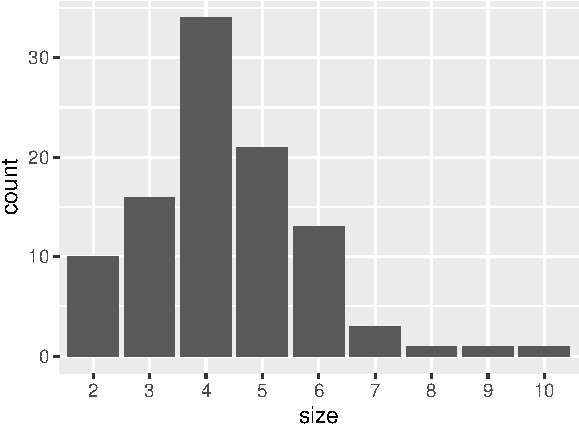
\includegraphics{RforGradThesis_files/figure-latex/one variable barplot-1} \end{center}

1変数の分布を示す関数は\texttt{x}のみを指定すれば良いです(\texttt{y}は不要です)。
\texttt{geom\_bar()}は何も指定しなければ縦軸を観測数(count)にしてくれます。
ここでは家族の人数が4人が最も多く、以下5人、3人\ldots{}の順に多いことがわかります。

\subsection{ヒストグラム}\label{ux30d2ux30b9ux30c8ux30b0ux30e9ux30e0}

ここでは、1つの連続変数の分布を示すヒストグラムについて説明します。
例として、\texttt{saving}に含まれる年間収入\texttt{inc}をヒストグラムにしてみましょう。

\begin{Shaded}
\begin{Highlighting}[]
\NormalTok{saving }\OperatorTok
\StringTok{  }\KeywordTok{ggplot}\NormalTok{(}\KeywordTok{aes}\NormalTok{(}\DataTypeTok{x =}\NormalTok{ inc)) }\OperatorTok{+}
\StringTok{  }\KeywordTok{geom_histogram}\NormalTok{()}
\end{Highlighting}
\end{Shaded}

\begin{center}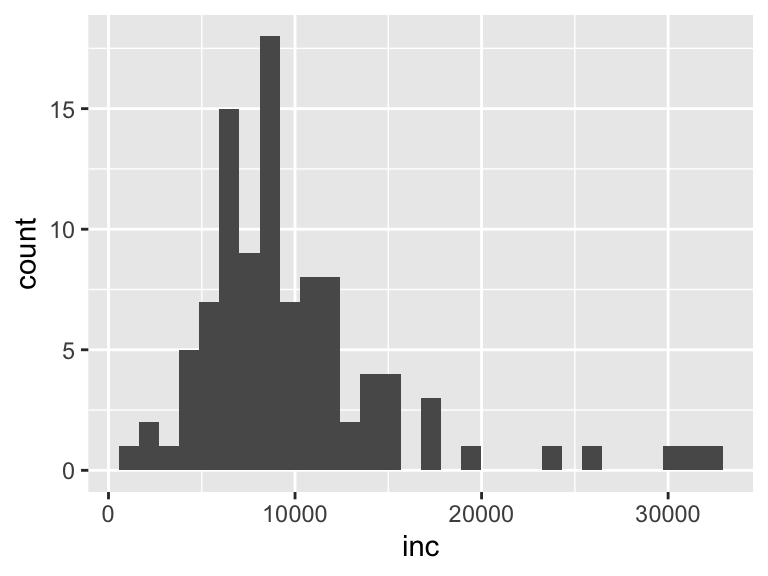
\includegraphics{RforGradThesis_files/figure-latex/one variable histogram-1} \end{center}

棒グラフと同じく\texttt{x}のみを指定すれば良く、縦軸は観測数になっています。
ヒストグラムで重要なのは、ビン(棒のことです)の数や幅です。
\texttt{geom\_histogram}はデフォルトでビンの数\texttt{bins}を30としていますが、見づらい場合は変えてみましょう。
例えば、ビンの数\texttt{bins}を15に減らしてみます。

\begin{Shaded}
\begin{Highlighting}[]
\NormalTok{saving }\OperatorTok
\StringTok{  }\KeywordTok{ggplot}\NormalTok{(}\KeywordTok{aes}\NormalTok{(}\DataTypeTok{x =}\NormalTok{ inc)) }\OperatorTok{+}
\StringTok{  }\KeywordTok{geom_histogram}\NormalTok{(}\DataTypeTok{bins =} \DecValTok{15}\NormalTok{) }\CommentTok{#ビンの数を15に指定}
\end{Highlighting}
\end{Shaded}

\begin{center}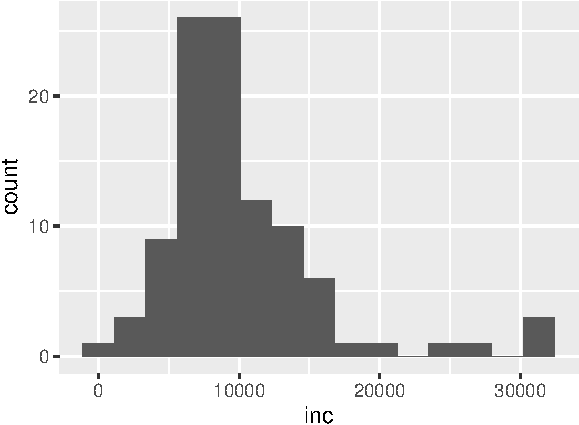
\includegraphics{RforGradThesis_files/figure-latex/one variable histogram bins-1} \end{center}

ビンの数が少なくなり分布が滑らかになりましたが、細かい情報が見えづらくなり一長一短です。
工夫したい方は、ビンの幅を定める\texttt{binwidth}や位置を定める\texttt{center}や\texttt{boundary}も活用してください。

\section{2変数の可視化}\label{ux5909ux6570ux306eux53efux8996ux5316-1}

変数と変数の関係の可視化は、研究結果を示すのに重要です。
2変数の場合、それぞれの変数の種類によって適切な図が異なります。

\begin{itemize}
\tightlist
\item
  連続変数と連続変数:散布図
\item
  連続変数とカテゴリ変数:散布図・棒グラフ・箱ひげ図
\item
  カテゴリ変数とカテゴリ変数:棒グラフ
\end{itemize}

\subsection{散布図}\label{ux6563ux5e03ux56f3}

連続変数と連続変数の関係を示すには、散布図が良いです。
散布図を描く関数が\texttt{geom\_point()}です。
ここでは、年齢\texttt{age}と年間貯蓄\texttt{inc}の関係を見てみましょう。

\begin{Shaded}
\begin{Highlighting}[]
\NormalTok{saving }\OperatorTok
\StringTok{  }\KeywordTok{ggplot}\NormalTok{(}\KeywordTok{aes}\NormalTok{(}\DataTypeTok{x =}\NormalTok{ age, }\DataTypeTok{y =}\NormalTok{ inc)) }\OperatorTok{+}
\StringTok{  }\KeywordTok{geom_point}\NormalTok{()}
\end{Highlighting}
\end{Shaded}

\begin{center}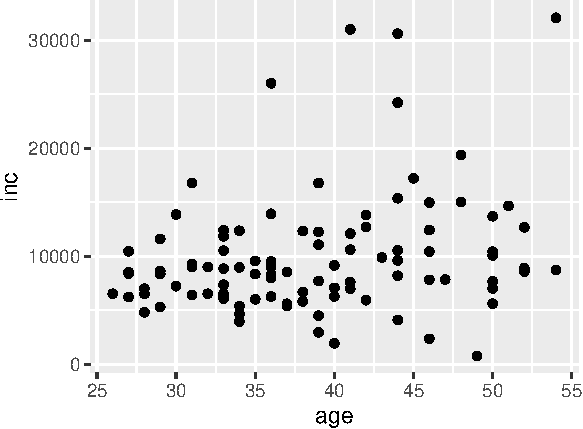
\includegraphics{RforGradThesis_files/figure-latex/geom_point-1} \end{center}

2変数なので、\texttt{x}と\texttt{y}を指定します。\texttt{x}が横軸、\texttt{y}が縦軸になり、通常は\texttt{x}が独立変数、\texttt{y}が従属変数となります。
散布図ではそれぞれの点が観測値となっています。
このデータでは、年齢と年間収入にはそこまで関係がないように見えます。

散布図に回帰分析で推定される回帰直線を足してみましょう。
回帰直線を描くコマンドは\texttt{geom\_smooth}です。

\begin{Shaded}
\begin{Highlighting}[]
\NormalTok{saving }\OperatorTok
\StringTok{  }\KeywordTok{ggplot}\NormalTok{(}\KeywordTok{aes}\NormalTok{(}\DataTypeTok{x =}\NormalTok{ age, }\DataTypeTok{y =}\NormalTok{ inc)) }\OperatorTok{+}
\StringTok{  }\KeywordTok{geom_point}\NormalTok{() }\OperatorTok{+}
\StringTok{  }\KeywordTok{geom_smooth}\NormalTok{(}\DataTypeTok{method =} \StringTok{"lm"}\NormalTok{, }\DataTypeTok{se =} \OtherTok{FALSE}\NormalTok{)}
\end{Highlighting}
\end{Shaded}

\begin{center}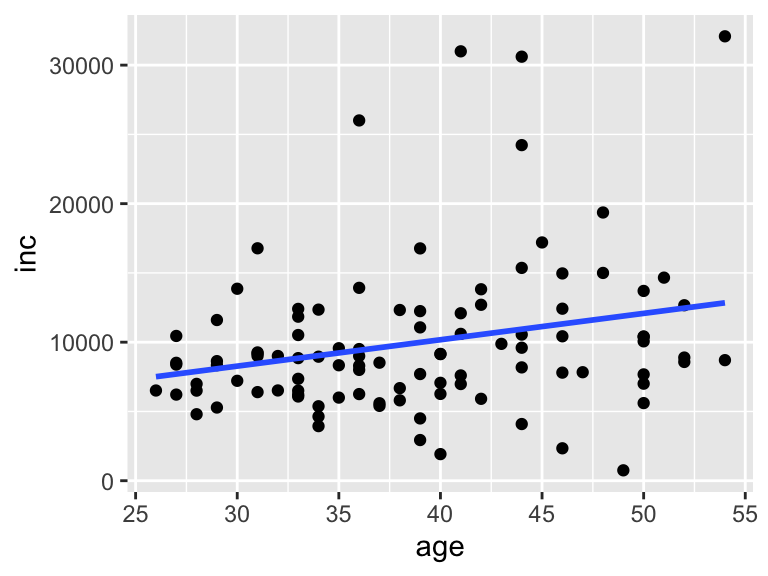
\includegraphics{RforGradThesis_files/figure-latex/add geom_smooth-1} \end{center}

ggplotはグラフを+でつなげて重ねることができます。ここでは、\texttt{geom\_point()}で散布図を描き、その上に\texttt{geom\_smooth()}で回帰直線を重ねています。
\texttt{geom\_smooth()}の引数\texttt{method}では、どのような線を描くのかを指定します。lmは線形モデル(linear
model)を指定しています。(指定しないと別の線になります)
\texttt{se}は標準偏差を見せる引数ですが、これをFALSEにして見せないようにしています。

カテゴリ変数と連続変数の関係を示すのにも、散布図を使うことができますが、弱点があります。
ここでは、教育年数\texttt{educ}から高卒以上のダミー変数\texttt{highschool}を作成した上で、年間収入\texttt{inc}の違いを見ていきましょう。

\begin{Shaded}
\begin{Highlighting}[]
\NormalTok{saving }\OperatorTok
\StringTok{  }\KeywordTok{mutate}\NormalTok{(}\DataTypeTok{highschool =} \KeywordTok{if_else}\NormalTok{(educ }\OperatorTok{>=}\StringTok{ }\DecValTok{12}\NormalTok{, }\DecValTok{1}\NormalTok{, }\DecValTok{0}\NormalTok{),}
         \DataTypeTok{highschool =} \KeywordTok{as_factor}\NormalTok{(highschool)) }\OperatorTok
\StringTok{  }\KeywordTok{ggplot}\NormalTok{(}\KeywordTok{aes}\NormalTok{(}\DataTypeTok{x =}\NormalTok{ highschool, }\DataTypeTok{y =}\NormalTok{ inc)) }\OperatorTok{+}
\StringTok{  }\KeywordTok{geom_point}\NormalTok{()}
\end{Highlighting}
\end{Shaded}

\begin{center}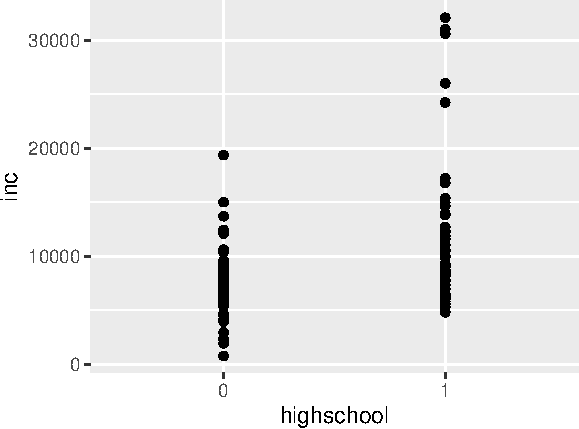
\includegraphics{RforGradThesis_files/figure-latex/geom_point category variable-1} \end{center}

散布図が書けました。しかし、点が固まってしまって見づらい図になってしまっています。
これを解決するには以下の方法があります。

\begin{itemize}
\tightlist
\item
  \texttt{geom\_point()}の代わりに\texttt{geom\_jitter()}を使う
\item
  散布図ではなく、棒グラフまたは箱ひげ図で代表値を図示する
\end{itemize}

\texttt{geom\_jitter()}は散布図の点をランダムに「散らして」表示する関数です。実際に見てみましょう。

\begin{Shaded}
\begin{Highlighting}[]
\NormalTok{saving }\OperatorTok
\StringTok{  }\KeywordTok{mutate}\NormalTok{(}\DataTypeTok{highschool =} \KeywordTok{if_else}\NormalTok{(educ }\OperatorTok{>=}\StringTok{ }\DecValTok{12}\NormalTok{, }\DecValTok{1}\NormalTok{, }\DecValTok{0}\NormalTok{),}
         \DataTypeTok{highschool =} \KeywordTok{as_factor}\NormalTok{(highschool)) }\OperatorTok
\StringTok{  }\KeywordTok{ggplot}\NormalTok{(}\KeywordTok{aes}\NormalTok{(}\DataTypeTok{x =}\NormalTok{ highschool, }\DataTypeTok{y =}\NormalTok{ inc)) }\OperatorTok{+}
\StringTok{  }\KeywordTok{geom_jitter}\NormalTok{(}\DataTypeTok{width =} \FloatTok{0.2}\NormalTok{)}
\end{Highlighting}
\end{Shaded}

\begin{center}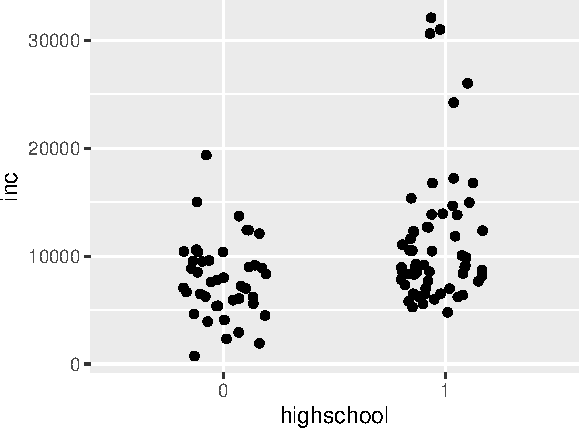
\includegraphics{RforGradThesis_files/figure-latex/geom_jitter category variable-1} \end{center}

これで多少見やすくなりました。\texttt{width\ =\ 0.2}では、散らす幅を指定しています。

\subsection{棒グラフ}\label{ux68d2ux30b0ux30e9ux30d5-1}

棒グラフでカテゴリごとの代表値を示したい場合は、\texttt{geom\_bar()}ではなく\texttt{stat\_summary()}を使います。
\texttt{stat\_summary()}の\texttt{fun.y}で使用したい代表値を(ここでは平均mean)、\texttt{geom}で表示方法ここでは棒グラフ\texttt{bar}を指定します。

\begin{Shaded}
\begin{Highlighting}[]
\NormalTok{saving }\OperatorTok
\StringTok{  }\KeywordTok{mutate}\NormalTok{(}\DataTypeTok{highschool =} \KeywordTok{if_else}\NormalTok{(educ }\OperatorTok{>=}\StringTok{ }\DecValTok{12}\NormalTok{, }\DecValTok{1}\NormalTok{, }\DecValTok{0}\NormalTok{),}
         \DataTypeTok{highschool =} \KeywordTok{as_factor}\NormalTok{(highschool)) }\OperatorTok
\StringTok{  }\KeywordTok{ggplot}\NormalTok{(}\KeywordTok{aes}\NormalTok{(}\DataTypeTok{x =}\NormalTok{ highschool, }\DataTypeTok{y =}\NormalTok{ inc)) }\OperatorTok{+}
\StringTok{  }\KeywordTok{stat_summary}\NormalTok{(}\DataTypeTok{fun.y =} \StringTok{"mean"}\NormalTok{, }\DataTypeTok{geom =} \StringTok{"bar"}\NormalTok{)}
\end{Highlighting}
\end{Shaded}

\begin{center}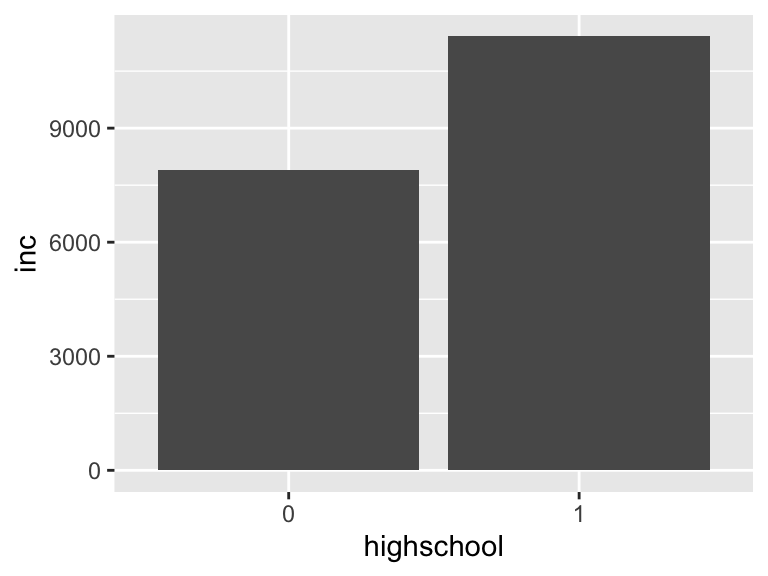
\includegraphics{RforGradThesis_files/figure-latex/stat_summary-1} \end{center}

これでカテゴリ別の平均値を棒グラフで示すことができました。

\subsection{箱ひげ図}\label{ux7bb1ux3072ux3052ux56f3}

箱ひげ図でカテゴリごとの代表値を示すこともできます。
箱ひげ図を描くには\texttt{geom\_boxplot}を用います。

\begin{Shaded}
\begin{Highlighting}[]
\NormalTok{saving }\OperatorTok
\StringTok{  }\KeywordTok{mutate}\NormalTok{(}\DataTypeTok{highschool =} \KeywordTok{if_else}\NormalTok{(educ }\OperatorTok{>=}\StringTok{ }\DecValTok{12}\NormalTok{, }\DecValTok{1}\NormalTok{, }\DecValTok{0}\NormalTok{),}
         \DataTypeTok{highschool =} \KeywordTok{as_factor}\NormalTok{(highschool)) }\OperatorTok
\StringTok{  }\KeywordTok{ggplot}\NormalTok{(}\KeywordTok{aes}\NormalTok{(}\DataTypeTok{x =}\NormalTok{ highschool, }\DataTypeTok{y =}\NormalTok{ inc)) }\OperatorTok{+}
\StringTok{  }\KeywordTok{geom_boxplot}\NormalTok{()}
\end{Highlighting}
\end{Shaded}

\begin{center}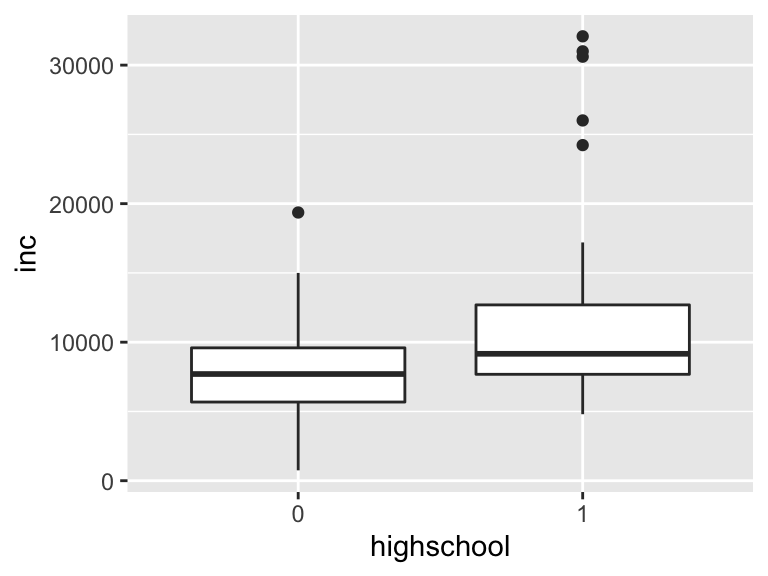
\includegraphics{RforGradThesis_files/figure-latex/geom_boxplot-1} \end{center}

箱ひげ図は以下のように読み取ります。

\begin{itemize}
\tightlist
\item
  白い箱の下辺:第一四分位(25\%点)
\item
  中央の太線:中央値(50\%点)
\item
  白い箱の上辺:第三四分位(75\%点)
\item
  箱の出ている線の長さ:1.5×IQR(第三四分位 - 第一四分位)
\item
  線の外側にある点:外れ値
\end{itemize}

なお、図を組み合わせることによりわかりやすくなるかもしれません。
\texttt{geom\_jitter()}による散布図と箱ひげ図を組み合わせてみましょう。
\texttt{ggplot2}では、\texttt{geom\_xxxx}を+でつなげることで、図を重ねることができます。

\begin{Shaded}
\begin{Highlighting}[]
\NormalTok{saving }\OperatorTok
\StringTok{  }\KeywordTok{mutate}\NormalTok{(}\DataTypeTok{highschool =} \KeywordTok{if_else}\NormalTok{(educ }\OperatorTok{>=}\StringTok{ }\DecValTok{12}\NormalTok{, }\DecValTok{1}\NormalTok{, }\DecValTok{0}\NormalTok{),}
         \DataTypeTok{highschool =} \KeywordTok{as_factor}\NormalTok{(highschool)) }\OperatorTok
\StringTok{  }\KeywordTok{ggplot}\NormalTok{(}\KeywordTok{aes}\NormalTok{(}\DataTypeTok{x =}\NormalTok{ highschool, }\DataTypeTok{y =}\NormalTok{ inc)) }\OperatorTok{+}
\StringTok{  }\KeywordTok{geom_boxplot}\NormalTok{(}\DataTypeTok{outlier.shape =} \OtherTok{NA}\NormalTok{) }\OperatorTok{+}\StringTok{ }\CommentTok{#外れ値を表示しないようオプションを設定}
\StringTok{  }\KeywordTok{geom_jitter}\NormalTok{(}\DataTypeTok{width =} \FloatTok{0.2}\NormalTok{)}
\end{Highlighting}
\end{Shaded}

\begin{center}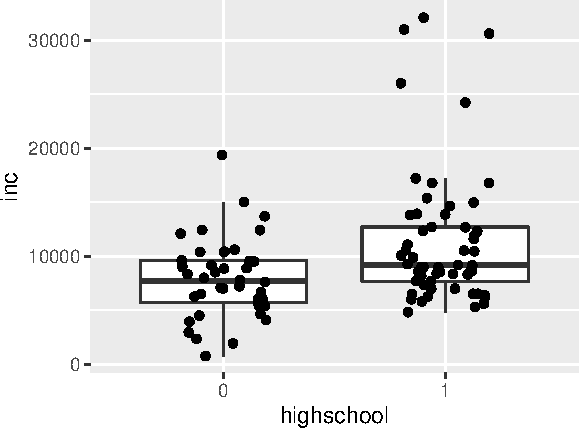
\includegraphics{RforGradThesis_files/figure-latex/geom_point and geom_boxplot-1} \end{center}

これでデータの全貌がわかりやすくなったでしょうか?

\chapter{t検定}\label{Ttest}

2群の平均値の差についての検定であるt検定を実施してみましょう。
t検定を行うコマンドは\texttt{t.test()}です。\texttt{t.test()}は以下のように記述します。

\begin{Shaded}
\begin{Highlighting}[]
\KeywordTok{t.test}\NormalTok{(従属変数 }\OperatorTok{~}\StringTok{ }\NormalTok{独立変数, }\DataTypeTok{data =}\NormalTok{ データフレーム名)}
\end{Highlighting}
\end{Shaded}

ここでは、\texttt{black}を用いて、黒人とそれ以外で年間収入\texttt{inc}に違いがあるかどうかを確認してみましょう。

\begin{Shaded}
\begin{Highlighting}[]
\KeywordTok{t.test}\NormalTok{(inc }\OperatorTok{~}\StringTok{ }\NormalTok{black, }\DataTypeTok{data =}\NormalTok{ saving)}
\end{Highlighting}
\end{Shaded}

\begin{verbatim}
## 
##  Welch Two Sample t-test
## 
## data:  inc by black
## t = 1.8562, df = 7.3906, p-value = 0.1036
## alternative hypothesis: true difference in means is not equal to 0
## 95 percent confidence interval:
##  -890.170 7726.938
## sample estimates:
## mean in group 0 mean in group 1 
##       10180.527        6762.143
\end{verbatim}

これでt検定を行うことができます。p値は\texttt{0.103}なので、今回は有意ではありませんでした。(差があるようには見えますが、黒人のサンプルが少ないことが影響していると思われます)

なお、\texttt{t.test()}はデフォルトで2群の分散が等しいと仮定しない「Welchのt検定」を実施します。
オプションで\texttt{var.equal\ =\ TRUE}とすれば分散が等しいと仮定した「スチューデントのt検定」が実施できますが、通常分散は異なることが多いため、デフォルトのままWelchのt検定を使用するのが良いでしょう。

t検定の結果はあまり見やすい形式にはなっていません。
\texttt{broom}というパッケージの関数\texttt{tidy}を使うと、結果を表形式で見やすくすることができます。
まずは\texttt{bloom}をインストールしておきましょう。

\begin{Shaded}
\begin{Highlighting}[]
\KeywordTok{install.packages}\NormalTok{(}\StringTok{"broom"}\NormalTok{)}
\end{Highlighting}
\end{Shaded}

その上で、\texttt{tidy()}を使ってみましょう。\texttt{t.test}の結果をパイプでつないで\texttt{tidy()}に渡してみます。

\begin{Shaded}
\begin{Highlighting}[]
\KeywordTok{library}\NormalTok{(broom)}
\KeywordTok{t.test}\NormalTok{(inc }\OperatorTok{~}\StringTok{ }\NormalTok{black, }\DataTypeTok{data =}\NormalTok{ saving) }\OperatorTok
\StringTok{  }\KeywordTok{tidy}\NormalTok{()}
\end{Highlighting}
\end{Shaded}

\begin{verbatim}
## # A tibble: 1 x 10
##   estimate estimate1 estimate2 statistic p.value parameter conf.low conf.high
##      <dbl>     <dbl>     <dbl>     <dbl>   <dbl>     <dbl>    <dbl>     <dbl>
## 1    3418.    10181.     6762.      1.86   0.104      7.39    -890.     7727.
## # ... with 2 more variables: method <chr>, alternative <chr>
\end{verbatim}

表示されている数値は以下のとおりです。

\begin{itemize}
\tightlist
\item
  \texttt{estimate}: 平均値の差
\item
  \texttt{estimate1}: グループ1の平均
\item
  \texttt{estimate2}: グループ2の平均
\item
  \texttt{statistic}: t値
\item
  \texttt{p.value}: p値
\item
  \texttt{parameter}: 自由度
\item
  \texttt{conf.low,\ conf.high}: 信頼区間の下限、上限
\item
  \texttt{method}: 使用した方法
\item
  \texttt{alternative}: 両側検定か片側検定か
\end{itemize}

\chapter{回帰分析}\label{Regression}

回帰分析とは、従属変数と独立変数の関係を数式(モデル)で表し、そのパラメータを推定する分析方法です。
ここでは、もっとも基本的な回帰分析である線形回帰(Linear
Regression)を扱います。

\section{線形回帰とは}\label{ux7ddaux5f62ux56deux5e30ux3068ux306f}

線形回帰では、従属変数 \(y\) と説明変数 \(x\) があるとき、\(y\) と \(x\)
の関係の以下の式(回帰式)で表します。

\(y = \alpha + \beta x\)

別の言い方をすると、 \(y\) を \(x\) の1次関数で表すと言うことです。
傾きを示す \(\beta\) は \(x\) と \(y\)
の関係を示す重要な数値で、係数(Coefficient)と呼ばれます。
これがプラスであれば \(x\) と \(y\)
に正の関係があることになりますし、マイナスであれば負の関係、0であれば関係がないことになります。
\(\beta\) は \(x\) が1単位高いとき、\(y\) が \(\beta\)
単位高い、という意味になります。
\textbf{回帰分析では変数の単位を常に把握して分析するよう心がけましょう。}

\(\alpha\) や \(\beta\) は最小二乗法(OLS)という方法で推定します。
この文書ではRでの操作方法に特化して説明するので、詳しくは各自調べてください。

\section{Rでの線形回帰}\label{rux3067ux306eux7ddaux5f62ux56deux5e30}

Rでは回帰式を\texttt{y\ \textasciitilde{}\ x}と表記します。(ここはChapter
\ref{Ttest}で学んだとt検定同じ表記です)
線形回帰を行う関数が\texttt{lm()}で(lmはlinear
modelの略)、以下のように表記します。

\begin{Shaded}
\begin{Highlighting}[]
\KeywordTok{lm}\NormalTok{(回帰式, }\DataTypeTok{data =}\NormalTok{ データフレーム)}
\end{Highlighting}
\end{Shaded}

例として、従属変数を年収\texttt{inc}、独立変数を教育年数\texttt{educ}とした線形回帰分析を行ってみましょう。
回帰式は \(inc = \alpha + \beta educ\) です。

\begin{Shaded}
\begin{Highlighting}[]
\KeywordTok{lm}\NormalTok{(inc }\OperatorTok{~}\StringTok{ }\NormalTok{educ, }\DataTypeTok{data =}\NormalTok{ saving)}
\end{Highlighting}
\end{Shaded}

\begin{verbatim}
## 
## Call:
## lm(formula = inc ~ educ, data = saving)
## 
## Coefficients:
## (Intercept)         educ  
##      1342.7        742.5
\end{verbatim}

Coefficientsのinterceptが\(\alpha\)、educが\(\beta\)を表します。
\(\beta\)を見ると、教育年数が1年高いと年収が742.5ドル高くなっていることがわかります。

\texttt{lm()}を実施すると、以上のように係数の推定値を得ることができますが、統計的推測のための数値(t値、p値)がわかりません。
\texttt{lm()}の結果を\texttt{summary()}に渡すと、詳細を見ることができます。

\begin{Shaded}
\begin{Highlighting}[]
\KeywordTok{lm}\NormalTok{(inc }\OperatorTok{~}\StringTok{ }\NormalTok{educ, }\DataTypeTok{data =}\NormalTok{ saving) }\OperatorTok
\StringTok{  }\KeywordTok{summary}\NormalTok{()}
\end{Highlighting}
\end{Shaded}

\begin{verbatim}
## 
## Call:
## lm(formula = inc ~ educ, data = saving)
## 
## Residuals:
##    Min     1Q Median     3Q    Max 
##  -7570  -3297  -1288   1617  20743 
## 
## Coefficients:
##             Estimate Std. Error t value Pr(>|t|)    
## (Intercept)   1342.7     1763.5   0.761    0.448    
## educ           742.5      146.1   5.084 1.78e-06 ***
## ---
## Signif. codes:  0 '***' 0.001 '**' 0.01 '*' 0.05 '.' 0.1 ' ' 1
## 
## Residual standard error: 4993 on 98 degrees of freedom
## Multiple R-squared:  0.2087, Adjusted R-squared:  0.2006 
## F-statistic: 25.84 on 1 and 98 DF,  p-value: 1.777e-06
\end{verbatim}

Coefficientsで以下の数値が表示されるようになりました。
それぞれの意味は教科書を確認してください。

\begin{itemize}
\tightlist
\item
  \texttt{Estimate}: 係数
\item
  \texttt{Std.\ Error}: 標準誤差
\item
  \texttt{t\ value}: t値
\item
  \texttt{Pr(\textgreater{}\textbar{}t\textbar{})}: p値
\end{itemize}

\texttt{educ}のp値は1.78e-06と表記されています。
これは、\(1.78 \times 10^{-6} = 1.78 \times 0.000001 = 0.00000178\)を表します。
とても小さい値なので、\texttt{educ}の係数 \(\beta\)
は有意に負と言えます。

他にも、決定係数 \(R^2\) などの数値も記載されています。

\texttt{summary()}で詳細を見ることができますが、やや見づらい印象があります。
表形式にするため、Chapter
\ref{Ttest}と同じく\texttt{broom}パッケージの関数\texttt{tidy()}を使ってみましょう。

\begin{Shaded}
\begin{Highlighting}[]
\KeywordTok{lm}\NormalTok{(inc }\OperatorTok{~}\StringTok{ }\NormalTok{educ, }\DataTypeTok{data =}\NormalTok{ saving) }\OperatorTok
\StringTok{  }\KeywordTok{tidy}\NormalTok{()}
\end{Highlighting}
\end{Shaded}

\begin{verbatim}
## # A tibble: 2 x 5
##   term        estimate std.error statistic    p.value
##   <chr>          <dbl>     <dbl>     <dbl>      <dbl>
## 1 (Intercept)    1343.     1764.     0.761 0.448     
## 2 educ            743.      146.     5.08  0.00000178
\end{verbatim}

表形式で見やすくなりました。

★練習問題

\begin{itemize}
\tightlist
\item
  収入\texttt{inc}を世帯人数\texttt{size}に回帰し、係数の意味を解釈してください。
\end{itemize}

\section{重回帰分析}\label{ux91cdux56deux5e30ux5206ux6790}

回帰分析には複数の説明変数を含め、それぞれの説明変数と被説明変数との変数を検証することができます。
複数の説明変数がある回帰分析を重回帰分析、一方上で説明した1つの説明変数がある回帰分析を単回帰分析と呼びます。
回帰式は説明変数を \(x_1, x_2\) としたとき、以下のようになります。

\(y = \alpha + \beta_1 x_1 + \beta_2 x_2\)

Rでの回帰式の表記は、\texttt{y\ \textasciitilde{}\ x1\ +\ x2}と、説明変数を\texttt{+}でつなげます。
ここでは、収入\texttt{inc}を教育年数\texttt{educ}と世帯人数\texttt{size}に回帰してみましょう。

\begin{Shaded}
\begin{Highlighting}[]
\KeywordTok{lm}\NormalTok{(inc }\OperatorTok{~}\StringTok{ }\NormalTok{educ }\OperatorTok{+}\StringTok{ }\NormalTok{size, }\DataTypeTok{data =}\NormalTok{ saving) }\OperatorTok
\StringTok{  }\KeywordTok{tidy}\NormalTok{()}
\end{Highlighting}
\end{Shaded}

\begin{verbatim}
## # A tibble: 3 x 5
##   term        estimate std.error statistic    p.value
##   <chr>          <dbl>     <dbl>     <dbl>      <dbl>
## 1 (Intercept)    3027.     2283.      1.33 0.188     
## 2 educ            743.      146.      5.10 0.00000171
## 3 size           -389.      335.     -1.16 0.249
\end{verbatim}

回帰式の解釈は単回帰分析と同様です。
ここでは、教育年数の結果は先ほどと大きく変わりませんでした。

説明変数はさらに3つ、4つ\ldots{}と増やすことができ、Rでは\texttt{y\ \textasciitilde{}\ x1\ +\ x2\ +\ x3\ +\ x4\ +\ ...}と\texttt{+}でつなげていきます。
説明変数が多く回帰式が長くなる場合は、回帰式を一旦オブジェクトとして保存しておくとコードが読みやすくなります。

例えば、上記の回帰分析にさらに年齢\texttt{age}、黒人ダミー\texttt{black}を加えてみましょう。

\begin{Shaded}
\begin{Highlighting}[]
\NormalTok{equation <-}\StringTok{ }\NormalTok{inc }\OperatorTok{~}\StringTok{ }\NormalTok{educ }\OperatorTok{+}\StringTok{ }\NormalTok{size }\OperatorTok{+}\StringTok{ }\NormalTok{age }\OperatorTok{+}\StringTok{ }\NormalTok{black}
\KeywordTok{lm}\NormalTok{(equation, }\DataTypeTok{data =}\NormalTok{ saving) }\OperatorTok
\StringTok{  }\KeywordTok{tidy}\NormalTok{()}
\end{Highlighting}
\end{Shaded}

\begin{verbatim}
## # A tibble: 5 x 5
##   term        estimate std.error statistic      p.value
##   <chr>          <dbl>     <dbl>     <dbl>        <dbl>
## 1 (Intercept)  -10005.    3934.     -2.54  0.0126      
## 2 educ            857.     144.      5.97  0.0000000408
## 3 size           -101.     320.     -0.317 0.752       
## 4 age             271.      66.3     4.09  0.0000917   
## 5 black          -553.    1878.     -0.294 0.769
\end{verbatim}

4つの説明変数による回帰分析の結果が出力できました。黒人ダミーの解釈については、次項をご覧ください。

★練習問題

\begin{itemize}
\tightlist
\item
  貯蓄額\texttt{sav}を被説明変数、教育年数\texttt{educ}、世帯人数\texttt{size}、年齢\texttt{age}を説明変数とする回帰分析を行い、それぞれの係数を解釈しなさい。
\end{itemize}

\section{ダミー変数の利用}\label{ux30c0ux30dfux30fcux5909ux6570ux306eux5229ux7528}

条件を満たすグループに1、条件を満たさないグループに0をとるダミー変数は、そのまま回帰分析に組み込むことができます。
ただし、解釈には注意が必要です。
ダミー変数の係数の解釈は、「条件を満たすグループは満たさないグループと比べて、被説明変数が(係数)大きい」となります。

ここでは、収入\texttt{inc}を黒人ダミー\texttt{black}に回帰してみましょう。

\begin{Shaded}
\begin{Highlighting}[]
\KeywordTok{lm}\NormalTok{(inc }\OperatorTok{~}\StringTok{ }\NormalTok{black, }\DataTypeTok{data =}\NormalTok{ saving)}
\end{Highlighting}
\end{Shaded}

\begin{verbatim}
## 
## Call:
## lm(formula = inc ~ black, data = saving)
## 
## Coefficients:
## (Intercept)        black  
##       10181        -3418
\end{verbatim}

黒人ダミーの係数は-3418です。これは、「黒人はそれ以外と比べて、年収が3418ドル低い」ことを意味します。

\section{カテゴリ変数の利用}\label{ux30abux30c6ux30b4ux30eaux5909ux6570ux306eux5229ux7528}

カテゴリ変数はそのまま回帰分析に組み込むことができません。
代わりにカテゴリの数-1個のダミー変数を作成し、回帰分析に組み込みます。
例えば、A, B, Cという3つのカテゴリがある場合、

\begin{itemize}
\tightlist
\item
  Bであれば1、そうでなければ0をとる「Bダミー」
\item
  Cであれば1、そうでなければ0をとる「Cダミー」
\end{itemize}

を作成し、回帰分析の独立変数として両方入れます。
係数の解釈には注意が必要です。それぞれの係数の解釈は、ダミー変数として入っていない「参照レベル」との比較となります。

\begin{itemize}
\tightlist
\item
  Bダミーの係数は「カテゴリBはカテゴリAと比べて被説明変数が(係数)大きい」
\item
  Cダミーの係数は「カテゴリCはカテゴリAと比べて被説明変数が(係数)大きい」
\end{itemize}

カテゴリBとカテゴリCを比べたい場合は、双方の係数を比較してください。

Rではカテゴリ変数がfactor型になっていれば、\textbf{自動的にダミー変数を作成して}回帰分析に入れてくれます。(もちろん、自分で作成しても構いませんし、そのほうが良い場合もあります)

ここでは、年齢のカテゴリ変数\texttt{age\_category}を作成し、年収\texttt{inc}に対する回帰分析に組み込んでみましょう。

\begin{Shaded}
\begin{Highlighting}[]
\NormalTok{saving_with_age_category <-}
\StringTok{  }\NormalTok{saving }\OperatorTok
\StringTok{    }\KeywordTok{mutate}\NormalTok{(}\DataTypeTok{age_category =} \KeywordTok{case_when}\NormalTok{(age }\OperatorTok{<}\StringTok{ }\DecValTok{30} \OperatorTok{~}\StringTok{ "20s"}\NormalTok{,}
\NormalTok{                                    age }\OperatorTok{>=}\StringTok{ }\DecValTok{30} \OperatorTok{&}\StringTok{ }\NormalTok{age }\OperatorTok{<}\StringTok{ }\DecValTok{40} \OperatorTok{~}\StringTok{ "30s"}\NormalTok{,}
\NormalTok{                                    age }\OperatorTok{>=}\StringTok{ }\DecValTok{40} \OperatorTok{&}\StringTok{ }\NormalTok{age }\OperatorTok{<}\StringTok{ }\DecValTok{50} \OperatorTok{~}\StringTok{ "40s"}\NormalTok{,}
\NormalTok{                                    age }\OperatorTok{>=}\StringTok{ }\DecValTok{50} \OperatorTok{~}\StringTok{ "50s"}
\NormalTok{                                    )}
\NormalTok{          )}

\KeywordTok{lm}\NormalTok{(inc }\OperatorTok{~}\StringTok{ }\NormalTok{age_category, }\DataTypeTok{data =}\NormalTok{ saving_with_age_category)}
\end{Highlighting}
\end{Shaded}

\begin{verbatim}
## 
## Call:
## lm(formula = inc ~ age_category, data = saving_with_age_category)
## 
## Coefficients:
##     (Intercept)  age_category30s  age_category40s  age_category50s  
##            7685             1330             3761             3885
\end{verbatim}

ここでは自動的に``20s''が参照レベルとなり、回帰分析には含まれていません。
各係数は20代と比べて収入がどれくらい高いかを表します。

\begin{itemize}
\tightlist
\item
  30代は20代より年収が1330ドル高い
\item
  40代は20代より年収が3761ドル高い
\item
  50代は20代より年収が3885ドル高い
\end{itemize}

それぞれ比較すると、年収は20代\textless{}30代\textless{}40代\textless{}50代と年齢が上がるにつれ高くなることがわかります。
しかし、40代と50代では差はほぼありません。

\section{交互作用の導入}\label{ux4ea4ux4e92ux4f5cux7528ux306eux5c0eux5165}

ある説明変数と被説明変数のとの関係が別の説明変数によって変化するような状況のことを交互作用がある、と言います。
例えば、収入と教育年数の関係が黒人ダミーによって異なる、といった場合です。
Rの回帰式では、交互作用は2つの変数を\texttt{:}でつなげることで表現できます。
上記の例をRで実施してみましょう。

\begin{Shaded}
\begin{Highlighting}[]
\KeywordTok{lm}\NormalTok{(inc }\OperatorTok{~}\StringTok{ }\NormalTok{educ }\OperatorTok{+}\StringTok{ }\NormalTok{black }\OperatorTok{+}\StringTok{ }\NormalTok{educ}\OperatorTok{:}\NormalTok{black, }\DataTypeTok{data =}\NormalTok{ saving) }\OperatorTok
\StringTok{  }\KeywordTok{tidy}\NormalTok{()}
\end{Highlighting}
\end{Shaded}

\begin{verbatim}
## # A tibble: 4 x 5
##   term        estimate std.error statistic   p.value
##   <chr>          <dbl>     <dbl>     <dbl>     <dbl>
## 1 (Intercept)   1595.      1926.    0.828  0.410    
## 2 educ           727.       157.    4.63   0.0000115
## 3 black         -525.      5773.   -0.0909 0.928    
## 4 educ:black     -63.1      615.   -0.103  0.918
\end{verbatim}

交互作用の解釈は少し複雑になります。
まずここでは教育年数\texttt{educ}の係数が727なので、教育年数1年高いと収入が727ドル高いことになります。
これは参照レベルである「黒人以外」での教育年数と収入の関係になります。

交互作用\texttt{educ:black}は-63ですが、これは黒人での教育年数と収入の係数が727-63=664であることを意味します。
なので、黒人では教育年数が1年高いと収入が664ドル高いということになります。
ただし、ここでは交互作用のp値が大きく有意ではありません。
すなわち、「黒人とそれ以外では教育年数と収入の関係が同じ」という仮説は棄却できていません。

交互作用の分析の際は、交互作用に使用した変数単体も必ず回帰式に含めるようにしてください。
\texttt{*}を使用すると、単体・相互作用をすべて自動的に作成・分析してくれます。

\begin{Shaded}
\begin{Highlighting}[]
\KeywordTok{lm}\NormalTok{(inc }\OperatorTok{~}\StringTok{ }\NormalTok{educ}\OperatorTok{*}\NormalTok{black, }\DataTypeTok{data =}\NormalTok{ saving) }\OperatorTok
\StringTok{  }\KeywordTok{tidy}\NormalTok{()}
\end{Highlighting}
\end{Shaded}

\begin{verbatim}
## # A tibble: 4 x 5
##   term        estimate std.error statistic   p.value
##   <chr>          <dbl>     <dbl>     <dbl>     <dbl>
## 1 (Intercept)   1595.      1926.    0.828  0.410    
## 2 educ           727.       157.    4.63   0.0000115
## 3 black         -525.      5773.   -0.0909 0.928    
## 4 educ:black     -63.1      615.   -0.103  0.918
\end{verbatim}

前の分析と全く同じ結果となっています。

★練習問題

\begin{itemize}
\tightlist
\item
  収入\texttt{inc}と年齢\texttt{age}の関係が黒人ダミーによって異なるかどうか、交互作用を含めた回帰分析を行い、その結果を解釈しなさい。
\end{itemize}

\section{回帰分析の表をまとめる}\label{ux56deux5e30ux5206ux6790ux306eux8868ux3092ux307eux3068ux3081ux308b}

ここまでは、回帰分析の結果は\texttt{tidy()}を用いて整理し、卒業論文に貼り付ける想定で話を進めてきました。
回帰分析の数が少ない場合は、この方法でも十分でしょう。

しかし、実施した回帰分析が多い場合、同じような表が続き冗長になります。
ここでは、\texttt{stargazer}パッケージを用いて、複数の回帰分析の結果をまとめた表を作成してみる方法を説明します。

以下の2つの回帰分析をまとめて表にしてみましょう。

\begin{enumerate}
\def\labelenumi{\arabic{enumi}.}
\tightlist
\item
  被説明変数を収入\texttt{inc}、説明変数を教育年数\texttt{educ}とする単回帰分析
\item
  被説明変数を収入\texttt{inc}、説明変数を教育年数\texttt{educ}と年齢\texttt{age}とする重回帰分析
\end{enumerate}

\texttt{stargazer()}では、回帰分析結果を保存したオブジェクト

\begin{Shaded}
\begin{Highlighting}[]
\NormalTok{regression1 <-}\StringTok{ }\KeywordTok{lm}\NormalTok{(inc }\OperatorTok{~}\StringTok{ }\NormalTok{educ, }\DataTypeTok{data =}\NormalTok{ saving) }\CommentTok{#単回帰分析の結果をオブジェクトに保存}
\NormalTok{regression2 <-}\StringTok{ }\KeywordTok{lm}\NormalTok{(inc }\OperatorTok{~}\StringTok{ }\NormalTok{educ }\OperatorTok{+}\StringTok{ }\NormalTok{age, }\DataTypeTok{data =}\NormalTok{ saving) }\CommentTok{#重回帰分析の結果をオブジェクトに保存}
\KeywordTok{stargazer}\NormalTok{(regression1, regression2, }\DataTypeTok{type =} \StringTok{"html"}\NormalTok{, }\DataTypeTok{out =} \StringTok{"test.doc"}\NormalTok{)}
\end{Highlighting}
\end{Shaded}

Dependent variable:

inc

(1)

(2)

educ

742.530***

869.852***

(146.062)

(137.566)

age

276.677***

(63.872)

Constant

1,342.745

-10,858.410***

(1,763.546)

(3,250.631)

Observations

100

100

R2

0.209

0.337

Adjusted R2

0.201

0.323

Residual Std. Error

4,992.593 (df = 98)

4,593.594 (df = 97)

F Statistic

25.844*** (df = 1; 98)

24.646*** (df = 2; 97)

Note:

\emph{p\textless{}0.1; \textbf{p\textless{}0.05; }}p\textless{}0.01

1・2行目では、\texttt{lm()}で回帰分析を行い、結果をオブジェクトとして\texttt{regression1},\texttt{regression2}にそれぞれ入力しています。
\texttt{stargazer()}では、表に含める回帰分析の結果を引数とし、さらにオプションを指定します。
\texttt{type}はデフォルトではLaTeXになっており多くの方は使えないと思いますので、ここではHTMLを指定して表形式に整えます。
\texttt{out}を指定すると、結果をファイルとして保存できます。
このファイルの表を卒業論文に貼り付け、必要に応じて加工すると良いでしょう。

表は列ごとに回帰分析の結果を示しています。
各行は説明変数を表し、かっこの無い上側が係数、かっこのある下側が標準誤差を表しています。
また、アスタリスク*で有意水準を表しています。
***が有意水準1\%で有意、**が有意水準5\%で有意、*が有意水準10\%で有意であることを示します。

線の下は以下のものを表しています。重要な情報なので、そのまま残しておきましょう。

\begin{itemize}
\tightlist
\item
  \texttt{Observation}: 観測数
\item
  \(R^2\): 決定係数
\item
  \texttt{Adjusted} \(R^2\): 修正済み決定係数
\item
  \texttt{Residual\ Std.\ Error}: 残差の標準誤差
\item
  \texttt{F\ Statistic}: F値(F検定の結果も合わせて表示)
\end{itemize}

\chapter{Wordファイルへの貼り付け}\label{Word}

多くの学生がWordで卒業論文を作成すると思われるので、Wordへ貼り付ける方法を説明します。
\textbf{Rで出た結果を目で見てWordに打ち込む方法は、タイプミスの危険がありおすすめしません。}

\section{表の貼り付け}\label{ux8868ux306eux8cbcux308aux4ed8ux3051}

Wordへ表を貼り付けるには様々な方法がありますが、ここではExcelを経由する方法を説明します。

\begin{itemize}
\tightlist
\item
  Rで作成した表をExcelにコピー&ペースト
\item
  貼り付けた部分を選択し、上のタブからデータ>区切り位置と選択
\item
  「固定長」を選び、次へ>次へ>完了

  \begin{itemize}
  \tightlist
  \item
    または、「区切り記号付き」→次へ>スペースにチェック→次へ>完了
  \end{itemize}
\item
  表形式になったので、形式を整えて(例.小数点以下の処理)Wordに貼り付け
\end{itemize}

RでWordの表を作成する方法としては、\texttt{flextable}パッケージなどを参照してください。(森もまだよくわかっておりません、情報募集中です)

\bibliography{book.bib,packages.bib}

\end{document}
